\documentclass[../notas medios.tex]{subfiles}

\begin{document}
\chapter{Equilibrio}

\graphicspath{{IMAGES/Cap4/}} 								 % Specifies the directory where pictures are stored


\subsection*{Coordenadas cilíndricas}


\begin{figure}[H]
\centering
	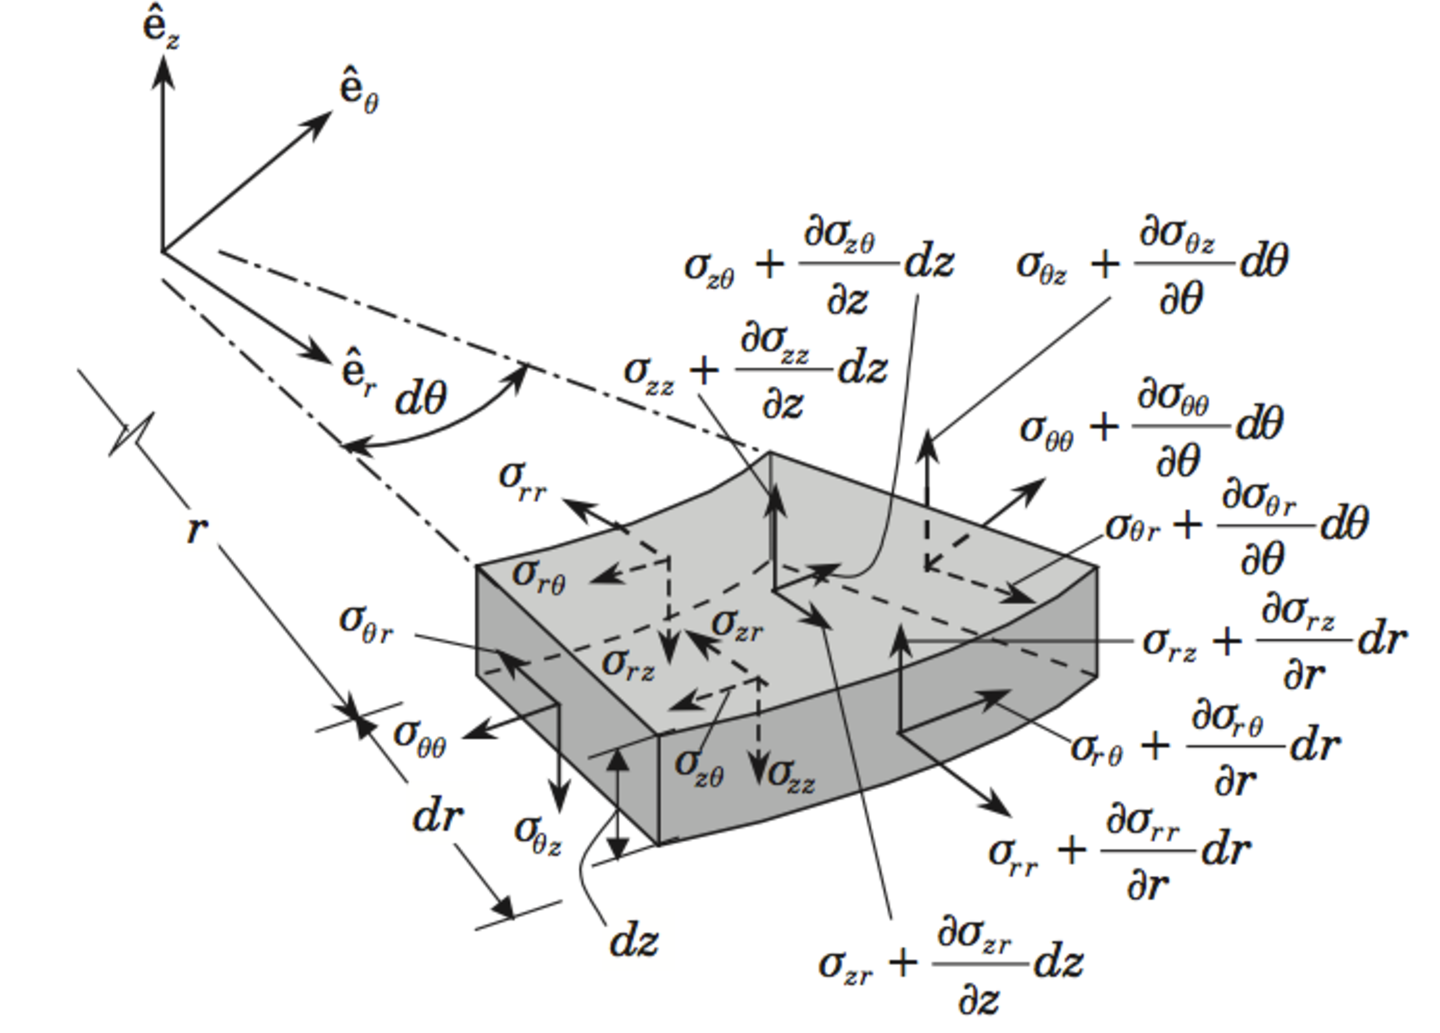
\includegraphics[width=4.0 in]{diffblockcil.pdf}
	\caption{Tensiones en un elemento diferencial de tamaño $dr{d\theta}dz$.}
	\label{diffcil}
\end{figure}

\begin{equation} \label{equcil}
\begin{split}
& \frac{{\partial {\sigma _{rr}}}}{{\partial r}} + \frac{1}{r}  \frac{{\partial {\tau _{{\theta}r}}}}{{\partial \theta}} + \frac{{\partial {\tau _{zr}}}}{{\partial z}} + \frac{\sigma _{rr} - \sigma _{{\theta}{\theta}}}{r} + {B_r} = 0 \\
& \frac{{\partial {\tau _{r{\theta}}}}}{{\partial r}} + \frac{1}{r} \frac{{\partial {\sigma _{{\theta}{\theta}}}}}{{\partial \theta}} + \frac{{\partial {\tau _{z{\theta}}}}}{{\partial z}} +  \frac{2 \tau_{r{\theta}}}{r} + {B_\theta} = 0 \\
& \frac{{\partial {\tau _{rz}}}}{{\partial r}} + \frac{1}{r} \frac{{\partial {\tau _{{\theta}z}}}}{{\partial \theta}} + \frac{{\partial {\sigma _{zz}}}}{{\partial z}} + \frac{ \tau_{rz}}{r} + {B_z} = 0 
\end{split}
\end{equation}

\subsection*{Ejemplo 1: Cuña autosoportada}

Considere la cuña doble de lado $\ell$ y ángulo interno $2 \phi$ mostrada en la \cref{WEDGE}. Se asume que esta se encuentra contenida en el plano $X-Y$, con condiciones de carga idealizables mediante un estado plano de tensiones (es decir 2D). La cuña se encuentra cargada por tracciones uniformes de intensidad $S$ aplicadas sobre sus 4 caras de tal manera que esta se encuentra auto-equilibrada. Determinar la solución al problema de valores en la frontera {\bf proponiendo una solución y verificando las condiciones de frontera}.

%
\begin{figure}[H]
\centering
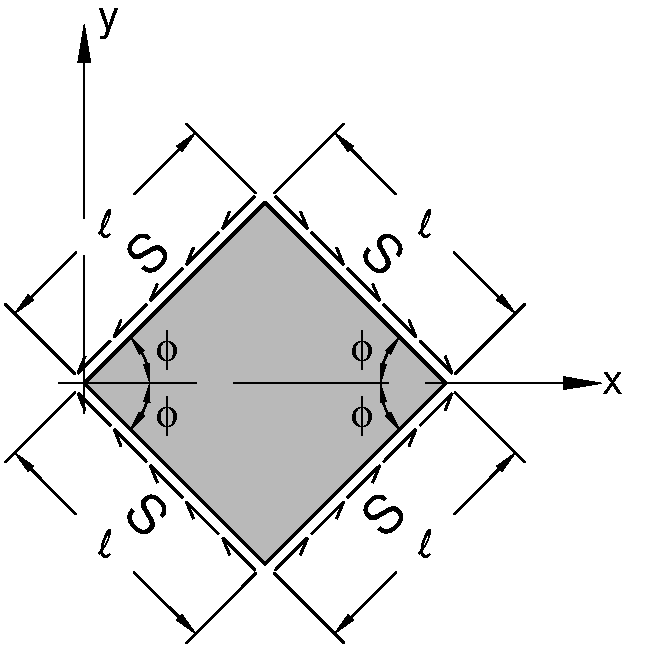
\includegraphics[width=8cm]{wedge.pdf}
\caption{2D Self-equilibrated wedge.}
\label{WEDGE}
\end{figure}

%
En el caso de estados de tensiones idealizables en 2 dimensiones y contenidos en el plano $x-y$ nada es función de $z$ y las ecuaciones de equlibrio \cref{equtr} y \cref{equrot} se reducen a;

\begin{equation}
\begin{aligned}
&\dfrac{\partial\sigma_{xx}}{\partial x}+\dfrac{\partial\tau_{xy}}{\partial y}=0\\
&\dfrac{\partial\tau_{xy}}{\partial x}+\dfrac{\partial\sigma_{yy}}{\partial y}=0
\end{aligned}
\label{equilibrium}
\end{equation}

mientras que el equlibrio rotacional se reduce a;

\[{\tau _{xy}} = {\tau _{yx}}.\]

Para proponer una solución planteamos las ecuaciones de equlibrio global de la cuña, lo cual es equivalente a asumir que las solución es constante. Se tiene entonces que;


\[\sum F_x=0 \longrightarrow -\ell C_\phi S+\sigma_{xx}\ell S_\phi=0\]\\
\[\sum F_y=0 \longrightarrow -\ell S_\phi S-\sigma_{yy}\ell C_\phi=0\] 

de donde resulta la siguiente función para el campo de tensiones;

\begin{equation}
\begin{aligned}
\sigma_{xx}&=SCot\phi\\
\sigma_{yy}&=-STan\phi\\
\tau_{xy}&=0
\end{aligned}
\label{solution}
\end{equation}

con la condición $\tau_{xy}=0$ debida a la simetría del problema.
\\
Para verificar que esta solución satisface las ecuaciones gobernantes reemplazamos la \cref{solution} en \cref{equilibrium}, notando que en este problema en particular no hay fuerzas de cuerpo ($\vec B = 0$)  resultando en;

\[\frac{{\partial (SCo{t_\phi })}}{{\partial x}} = 0\]

y

\[\frac{{\partial ( - STa{n_\phi })}}{{\partial y}} = 0.\]


Sin embargo es claro que existen infinitas funciones $\sigma  = \sigma (x,y)$  que satisafacen las \cref{equilibrium} y para garantizar que la solución {\bf propuesta} es la solución correcta al problema es necesario verificar que esta satisface además las condiciones de frontera del problema.

Sean $\hat{n}^1$,$\hat{n}^2$,$\hat{n}^3$,$\hat{n}^4$ los vectores normales externos a las caras expuestas de la cuña y escritos en el sistema de referencia $x-y$ como;

\[\hat{n}^1=-S_{\phi}\hat{e}_{x}+C_{\phi}\hat{e}_{y}\]
\[\hat{n}^2=-S_{\phi}\hat{e}_{x}-C_{\phi}\hat{e}_{y}\]
\[\hat{n}^3=+S_{\phi}\hat{e}_{x}+C_{\phi}\hat{e}_{y}\]
\[\hat{n}^4=+S_{\phi}\hat{e}_{x}-C_{\phi}\hat{e}_{y}.\]


Para calcular las componentes del vector de tracciones sobre cada una de las caras usamos la fórmula de Cauchy escrita como;

\[t_{i}=\sigma_{ij}\hat{n}_{j}.\]

Luego, sobre la cara con vector normal $\hat{n}^1$ tenemos;

\[t_{x}=-SC_{\phi}\]
\[t_{y}=-SS_{\phi}\]

similarmente sobre la cara con vector normal $\hat{n}^2$

\[t_{x}=-SC_{\phi}\]
\[t_{y}=+SS_{\phi}\]

sobre la cara con vector normal $\hat{n}^3$ 

\[t_{x}=+SC_{\phi}\]
\[t_{y}=-SS_{\phi}\]

y finalmente, sobre la cara con vector normal $\hat{n}^4$;

\[t_{x}=+SC_{\phi}\]
\[t_{y}=+SS_{\phi}\]

los cuales coinciden con las tracciones especificadas como condiciones de frontera del problema.


\subsection*{Ejemplo 2: Empujes sobre presa de concreto}

Si se sabe que la función de tensiones dada en la \cref{sln1} es solución al problema de valores en la frontera del medio continuo sobre el dominio mostrado en la \cref{dam}, en donde $\gamma$ es una constante\footnote{Un script .py con las funciones de esfuerzo está disponible en:  {\url{https://github.com/casierraa/MMC/blob/master/dam.py}}} . Se pide: 

\begin{equation}
\begin{split}
{\sigma _{xx}} & = \gamma x - 2\gamma y \\
{\sigma _{yy}} & =  - \gamma x \\
{\tau _{xy}}   & =  - \gamma y
\end{split}
\label{sln1}
\end{equation}

\begin{figure}[H]
\centering
	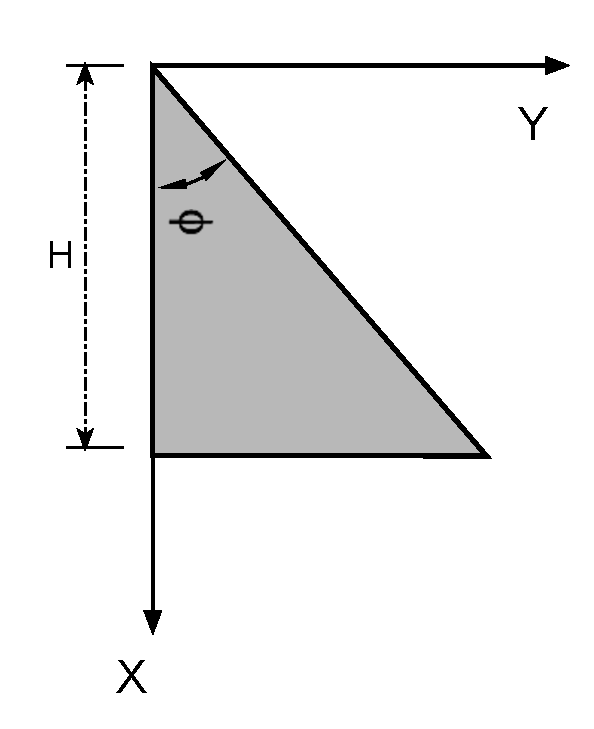
\includegraphics[width=2.5 in]{dam.pdf}
	\caption{Dominio de validez de la solución.}
	\label{dam}
\end{figure}


\begin{itemize}
\item[•] Identificar la frontera del problema.
\item[•] Verificar que la función dada en la \cref{sln1} efectivamente satisface las condiciones de equilibrio local.
\item[•] Determinar las condiciones de frontera sobre el dominio (graficar).
\item[•] Verificar que la solución satisface condiciones de equilibrio global.
\end{itemize}


\subsubsection*{Solución}
Sustituyendo la solución dada en \cref{sln1} en las ecuaciones de equilibrio local y considerando que $B_x =0$ y $B_y =0$ se verifica que la solución satisface equilibrio;

\[\frac{{\partial (\gamma x - 2\gamma y)}}{{\partial x}} + \frac{{\partial ( - \gamma y)}}{{\partial y}} + {B_x} = 0\]
\[\gamma  - \gamma  = 0\] 
\[\frac{{\partial ( - \gamma y)}}{{\partial x}} + \frac{{\partial ( - \gamma x)}}{{\partial y}} + {B_y} = 0\]
\[0 + 0 = 0.\]

Sean los vectores normales a las caras vertical, horizontal e inclinada ${{\hat n}^1} =  - \hat j$, ${{\hat n}^2} =   \hat i$ y ${{\hat n}^3} =  - {S_\phi }\hat i + {C_\phi }\hat j$ respectivamente. En la superficie con normal ${{\hat n}^1}$ ($y=0$) se tiene que;
\[{\sigma _{xx}} = \gamma x\]
\[{\sigma _{yy}} =  - \gamma x\]
y
\[{\tau _{xy}} = 0 \]

luego;

\[\left\{ {\begin{array}{*{20}{c}}
{{t_x}}\\
{{t_y}}
\end{array}} \right\} = \left[ {\begin{array}{*{20}{c}}
{\gamma x}&0\\
0&{ - \gamma x}
\end{array}} \right]\left\{ {\begin{array}{*{20}{c}}
0\\
{ - 1}
\end{array}} \right\} = \left\{ {\begin{array}{*{20}{c}}
0\\
{\gamma x}
\end{array}} \right\}\]

esta distribución se muestra en la \cref{sigy};


\begin{figure}[H]
\centering
	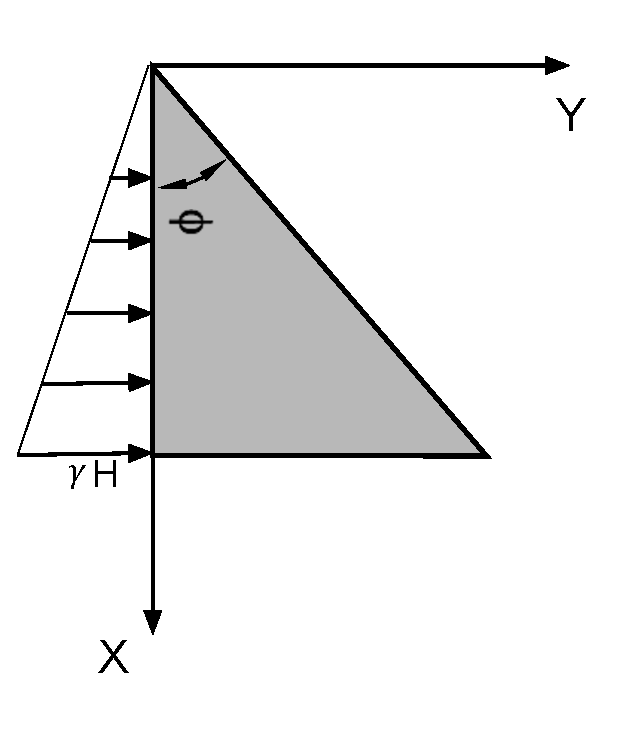
\includegraphics[width=2.0 in]{sigy.pdf}
	\caption{Distribución de tracciones sobre la cara vertical.}
	\label{sigx}
\end{figure}


Similarmente, sobre la superficie con normal ${{\hat n}^2} =   \hat i$ ($x=H$) se tiene;

\[{\sigma _{xx}} = \gamma H - 2\gamma y\]
\[{\sigma _{yy}} =  - \gamma H\]
y
\[{\tau _{xy}} =  - \gamma y\]
luego;

\[\left\{ {\begin{array}{*{20}{c}}
{{t_x}}\\
{{t_y}}
\end{array}} \right\} = \left[ {\begin{array}{*{20}{c}}
{\gamma H - 2\gamma y}&{ - \gamma y}\\
{ - \gamma y}&{ - \gamma H}
\end{array}} \right]\left\{ {\begin{array}{*{20}{c}}
1\\
0
\end{array}} \right\} = \left\{ {\begin{array}{*{20}{c}}
{\gamma H - 2\gamma y}\\
{ - \gamma y}
\end{array}} \right\}.\]


La distribución de la componente $t_x$ sobre esta cara, corresponde a la tensión normal $\sigma_{xx}$ tal y como se muestra en la \cref{sigx}. 

\begin{figure}[H]
\centering
	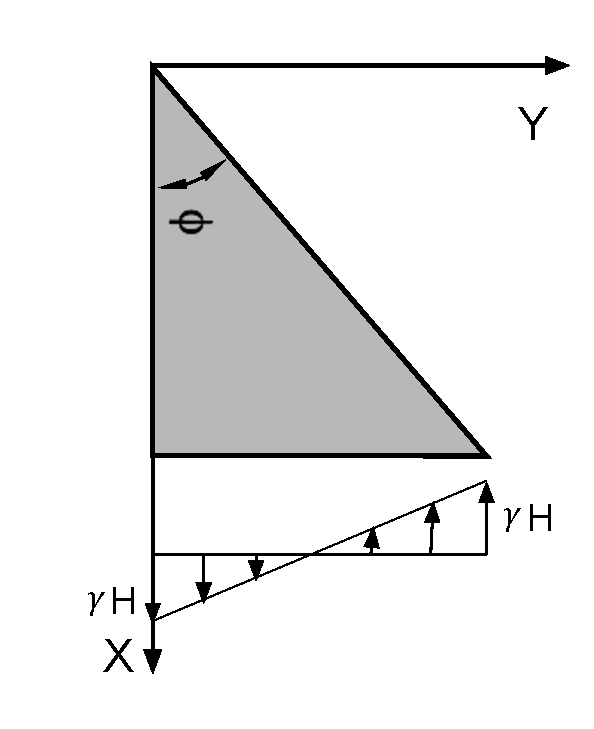
\includegraphics[width=2.0 in]{sigx.pdf}
	\caption{Distribución de tensiones normales sobre la cara horizontal.}
	\label{sigy}
\end{figure}

Similarmente, la componente $t_y$ corresponde a la componente $\tau_{xy}$. Sobre esta cara se tiene en $y=0$  que $t_y = 0$, mientras que en $y=H$ $t_y = - \gamma H$. Esta distribución se muestra en la \cref{taoxy};

\begin{figure}[H]
\centering
	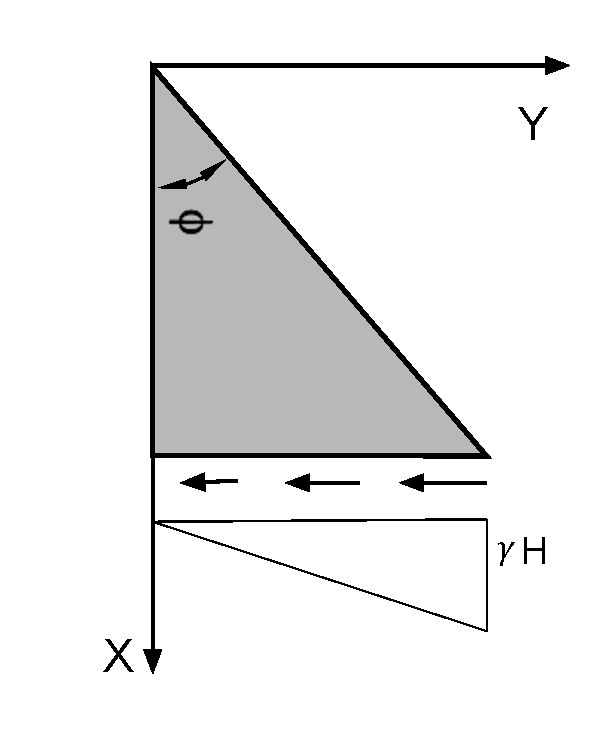
\includegraphics[width=2.0 in]{tauxy.pdf}
	\caption{Distribución de tensiones cortantes sobre la cara horizontal.}
	\label{taoxy}
\end{figure}


La solución para la presa se ha implementado en el script de python dam.py distribuido en EAFIT interactiva. En la \cref{Sx}, \cref{Sy}, \cref{Txy} y \cref{Sc} se peresenta la distribución de tensiones sobre toda la presa en forma de contornos o curvas de nivel de isotensiones (igual valor de tensión)

\begin{figure}[H]
     \centering
     \subfloat[Esfuerzo axial en x]{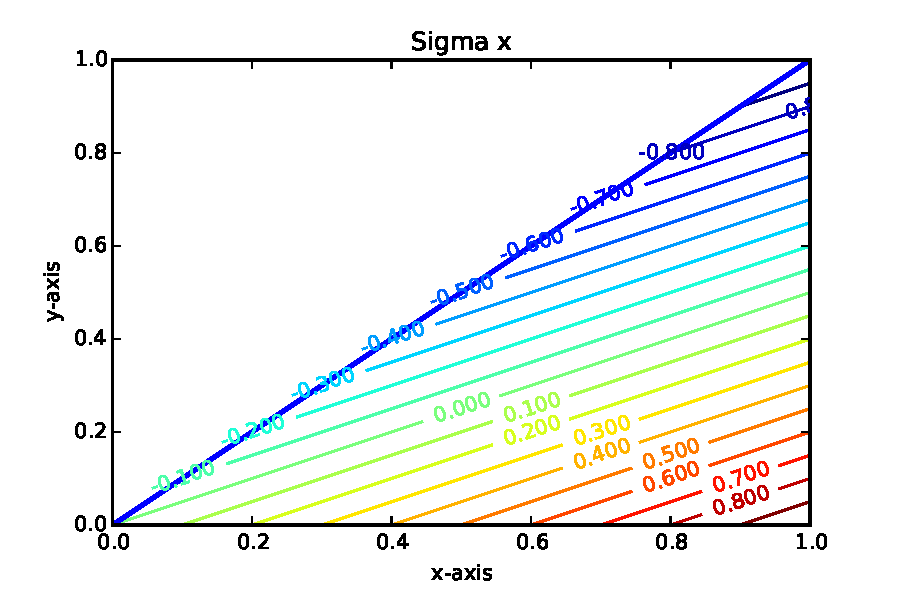
\includegraphics[width=2.2 in]{sigmax.pdf}\label{Sx}}
     \hspace{0.5cm}
     \subfloat[Esfuerzo axial en y]{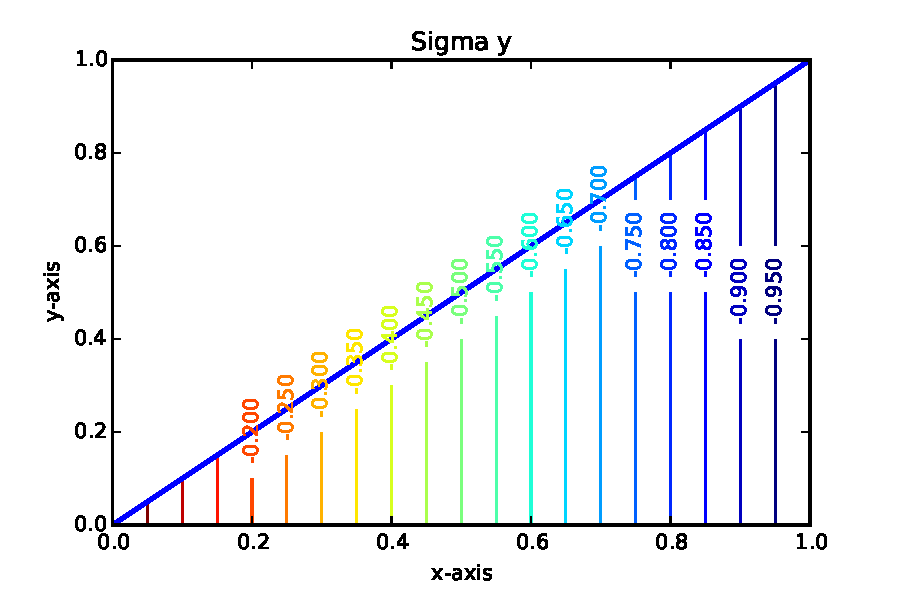
\includegraphics[width=2.2 in]{sigmay.pdf}\label{Sy}}\\
     \subfloat[Esfuerzo cortante]{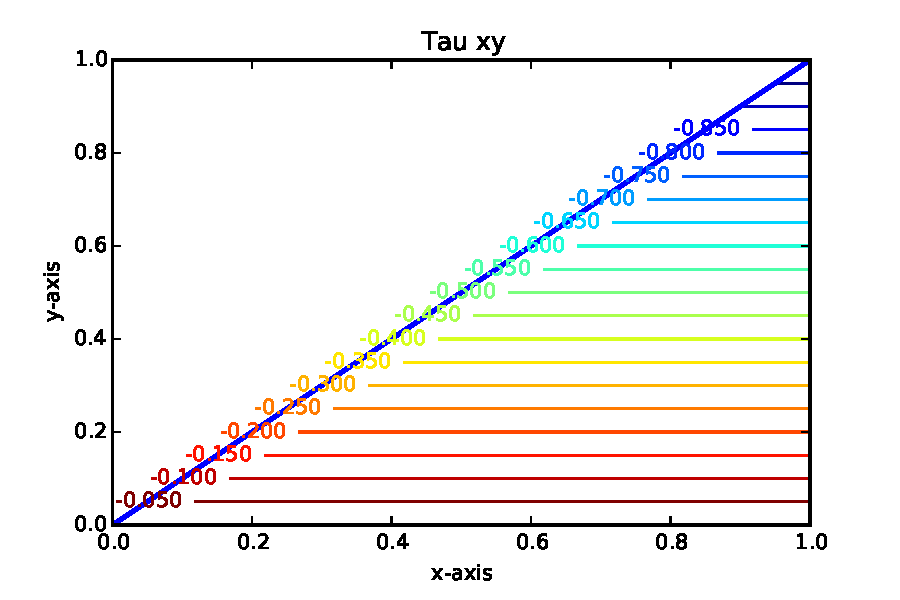
\includegraphics[width=2.2 in]{taoxy.pdf}\label{Txy}}
     \hspace{0.5cm}
     \subfloat[Esfuerzo cortante máximo]{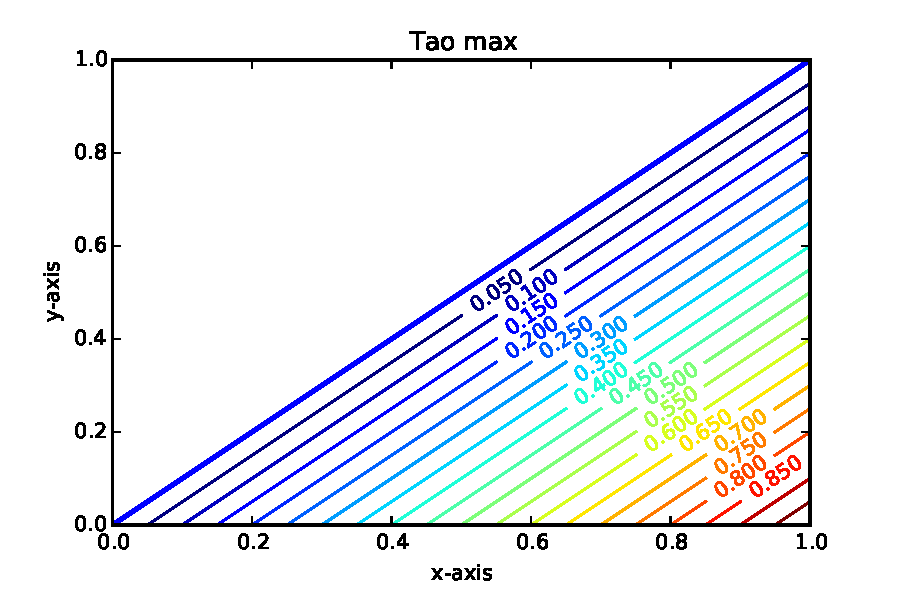
\includegraphics[width=2.2 in]{sigmac.pdf}\label{Sc}}\\
     \caption{Variación de las tensiones que producen fuerzas en la dirección $x$ y $y$ sobre la presa.}
     \label{python}
\end{figure}


Para verificar el equilibrio global consideremos el diagrama de cuerpo libre mostrado en la \cref{dcl}

\begin{figure}[H]
\centering
	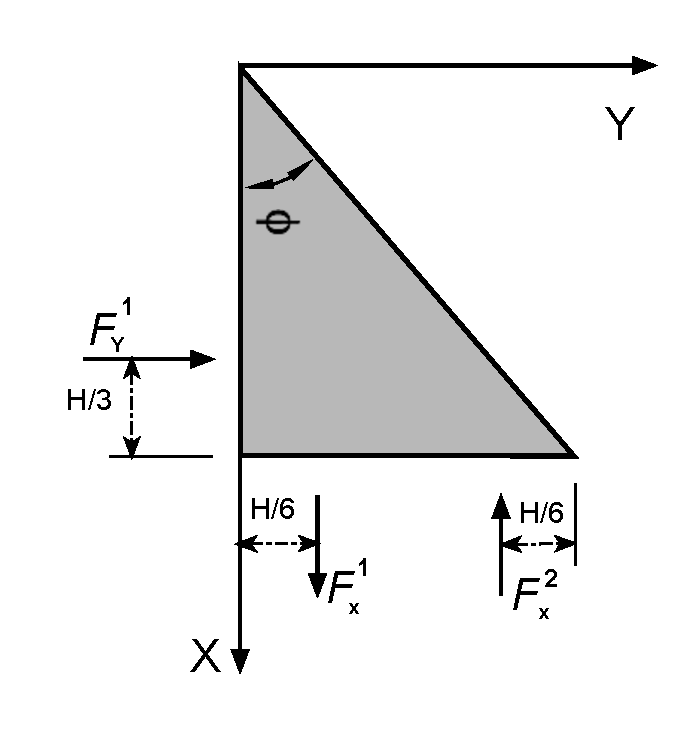
\includegraphics[width=3.0 in]{fbodydam.pdf}
	\caption{Diagrama de cuerpo libre de la presa.}
	\label{dcl}
\end{figure}


donde;
\[F_x^1 = \frac{{\gamma {H^2}}}{4}\]
\[F_x^2 =  - \frac{{\gamma {H^2}}}{4}\]
luego
\[\sum {{F_x} = 0} \]
y
\[F_y^1 = \frac{{\gamma {H^2}}}{2}\]
luego
\[\sum {{F_y} = 0} \]
similarmente
\[\sum {{M_A} = } \frac{4}{{24}}\gamma {H^3} + \frac{1}{{24}}\gamma {H^3} - \frac{5}{{24}}\gamma {H^3} = 0\]
con lo que se verifica que la solución satisface equilibrio global.



\section*{Soluciones clásicas para sólidos}
En esta sección se presentan algunas soluciones clásicas en términos de tensiones. Se inivta al estudiante a realizar el análisis de las mismas usando razonamientos similares a los presentados en los 2 ejemplos anteriores y de acuerdo con los objetivos de aprendizaje declarados al inicio del capitulo.

\subsection*{Barra prismática soportada en la superficie superior y sometida a la acción de su propio peso}

La barra prismatica mostrada en la \cref{barra}

\begin{figure}[H]
\centering
	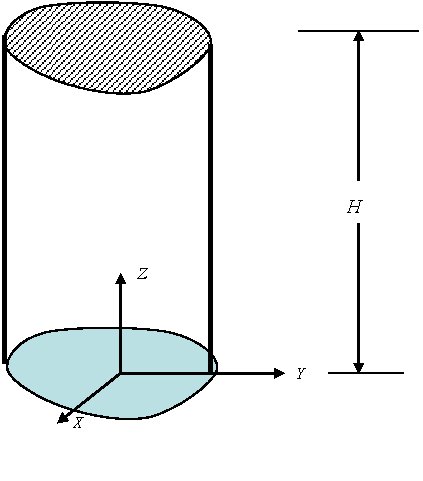
\includegraphics[width=2.5 in]{barrapp.pdf}
	\caption{Barra prismática sometica a la acción de peso propio.}
	\label{barra}
\end{figure}

se encuentra atada sobre la superficie superior y esta sometida a la acción de su propio peso. La función dada en la \cref{slnb} es la solución del problema,


\begin{equation}
\begin{split}
{\sigma _{zz}} & = \gamma z \\
{\sigma _{xx}} & = {\sigma _{yy}} = 0 \\
{\tau _{xy}}   & = {\tau _{xz}} = {\tau _{yz}} = 0
\end{split}
\label{slnb}
\end{equation}


\subsection*{Viga en voladizo}

La \cref{Viga} muestra una viga cantiliver sometida a una carga $P$ en uno de sus extremos: 
\begin{figure}[H]
\centering
	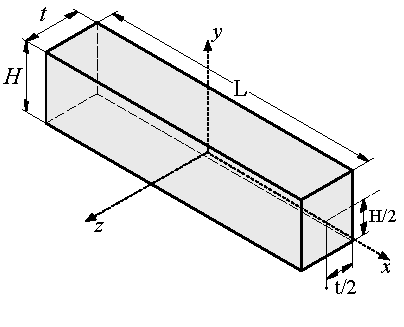
\includegraphics[width=3.0 in]{Viga.pdf}
	\caption{Viga cantiliver}
	\label{Viga}
\end{figure}

El tensor solución se da en la \cref{slnc}.

\begin{equation}
\begin{split}
{\sigma_{xx}} & = - \dfrac{P}{I} (XY) \\
 {\sigma_{yy} }&= \sigma_{zz} = 0 \\
{\tau_{xy}} & = \tau_{yx} = - \dfrac{P}{2I} (\dfrac{H^2}{4} - Y^2) \\ 
{\tau_{xz}} &= 0
\end{split}	
\label{viga}
\end{equation}


\subsection*{Cilindro sometido a presión interna y externa}
Para este problema se requiren las ecuaciones de equlibrio local en coordenadas polares dadas por:

\begin{equation} \label{equcil}
\begin{split}
& \frac{{\partial {\sigma _{rr}}}}{{\partial r}} + \frac{1}{r}\frac{{\partial {\tau _{\theta r}}}}{{\partial \theta }} + \frac{{{\sigma _{rr}} - {\sigma _{\theta \theta }}}}{r} + {B_r} = 0 \\
& \frac{{\partial {\tau _{\theta r}}}}{{\partial r}} + \frac{1}{r}\frac{{\partial {\sigma _{\theta \theta }}}}{{\partial \theta }} + \frac{{2{\tau _{r\theta }}}}{r} + {B_\theta } = 0
\end{split}
\end{equation}

La \cref{cilindro} muestra un cilindro de radio interno $a$ y radio externo $b$ sometido a presiones internas y externas $p_a$ y $p_b$ respectivamente. 

\begin{figure}[H]
\centering
	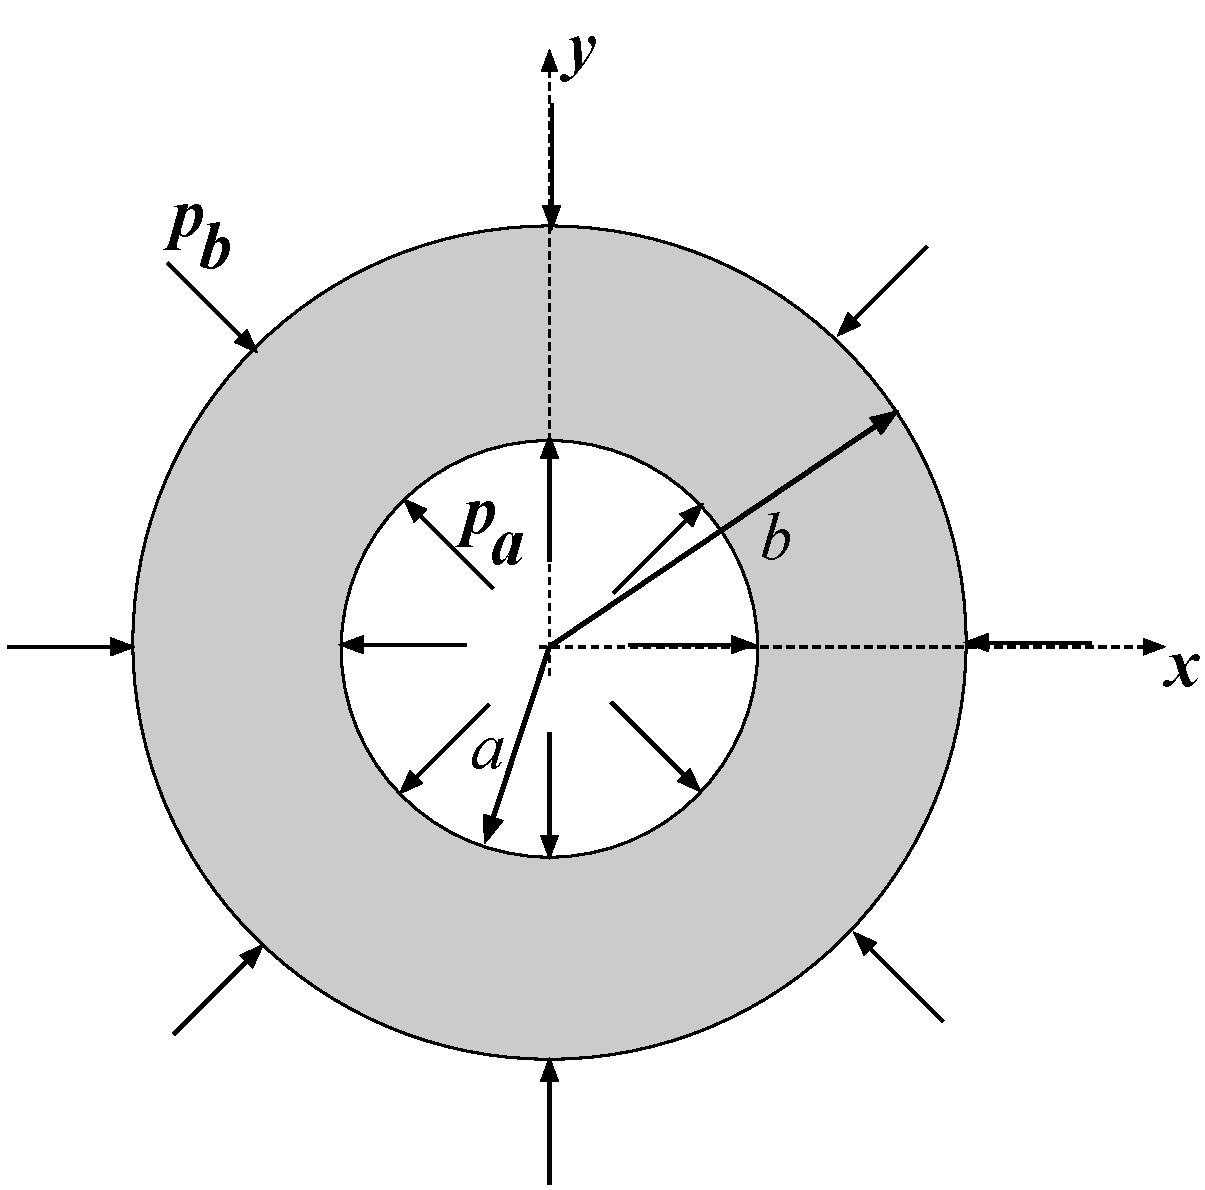
\includegraphics[width=3.0 in]{cilindro.pdf}
	\caption{Cilindro sometido a presión interna y externa.}
	\label{cilindro}
\end{figure}

El tensor solución se da en la \cref{slnc}.

\begin{equation}
\begin{split}
{\sigma _{rr}} & =  - \frac{{\left( {\frac{{{b^2}}}{{{r^2}}} - 1} \right)}}{{\left( {\frac{{{b^2}}}{{{a^2}}} - 1} \right)}}{p_a} - \frac{{\left( {1 - \frac{{{a^2}}}{{{r^2}}}} \right)}}{{\left( {1 - \frac{{{a^2}}}{{{b^2}}}} \right)}}{p_b} \\
{\sigma _{\theta \theta }} & = \frac{{\left( {\frac{{{b^2}}}{{{r^2}}} + 1} \right)}}{{\left( {\frac{{{b^2}}}{{{a^2}}} - 1} \right)}}{p_a} - \frac{{\left( {1 + \frac{{{a^2}}}{{{r^2}}}} \right)}}{{\left( {1 - \frac{{{a^2}}}{{{b^2}}}} \right)}}{p_b}
\end{split}
\label{slnc}
\end{equation}

\subsection*{Flamant}

La \cref{Flamant} muestra un semi-espacio sometido a una carga lineal superficial P. 

\begin{figure}[H]
\centering
	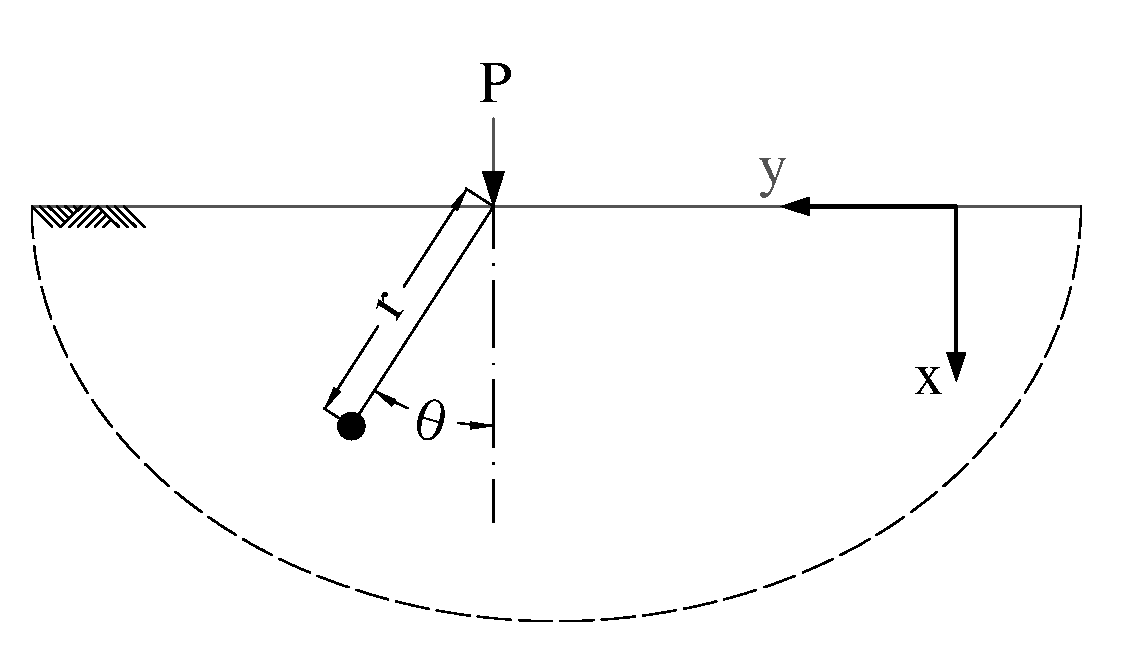
\includegraphics[width=3.0 in]{Bousinesq.pdf}
	\caption{Medio continuo sometido a una carga P.}
	\label{Flamant}
\end{figure}

El tensor solución se da en la \cref{slnf}

\begin{equation}
\begin{split}
{ \sigma_{rr}} & = -\dfrac{2P}{\pi r} Cos \theta \\
{\sigma_{\theta\theta}}  &= 0\\
{\tau_{r\theta}}&= 0
\end{split}
\label{slnf}
\end{equation}

\subsection*{Ejemplo 3: aplicación de solución para cilindro sometido a presión interna y externa}

\begin{enumerate} 

\item La solución para un cilindro de radio interno $a$ y radio externo $b$ sometido a presiones internas y externas $p_a$ y $p_b$ respectivamente (ver \cref{cilindro}), está dado por:

\begin{equation*}
\sigma _{rr}  =  - \frac{{\left( {\frac{{{b^2}}}{{{r^2}}} - 1} \right)}}{{\left( {\frac{{{b^2}}}{{{a^2}}} - 1} \right)}}{p_a} - \frac{{\left( {1 - \frac{{{a^2}}}{{{r^2}}}} \right)}}{{\left( {1 - \frac{{{a^2}}}{{{b^2}}}} \right)}}{p_b} \hspace{1.5cm}
\sigma _{\theta \theta } = \frac{{\left( {\frac{{{b^2}}}{{{r^2}}} + 1} \right)}}{{\left( {\frac{{{b^2}}}{{{a^2}}} - 1} \right)}}{p_a} - \frac{{\left( {1 + \frac{{{a^2}}}{{{r^2}}}} \right)}}{{\left( {1 - \frac{{{a^2}}}{{{b^2}}}} \right)}}{p_b} \hspace{1.5cm}
\tau _{r\theta} = 0
\label{slnc}
\end{equation*}

\begin{figure}[H]
\centering
	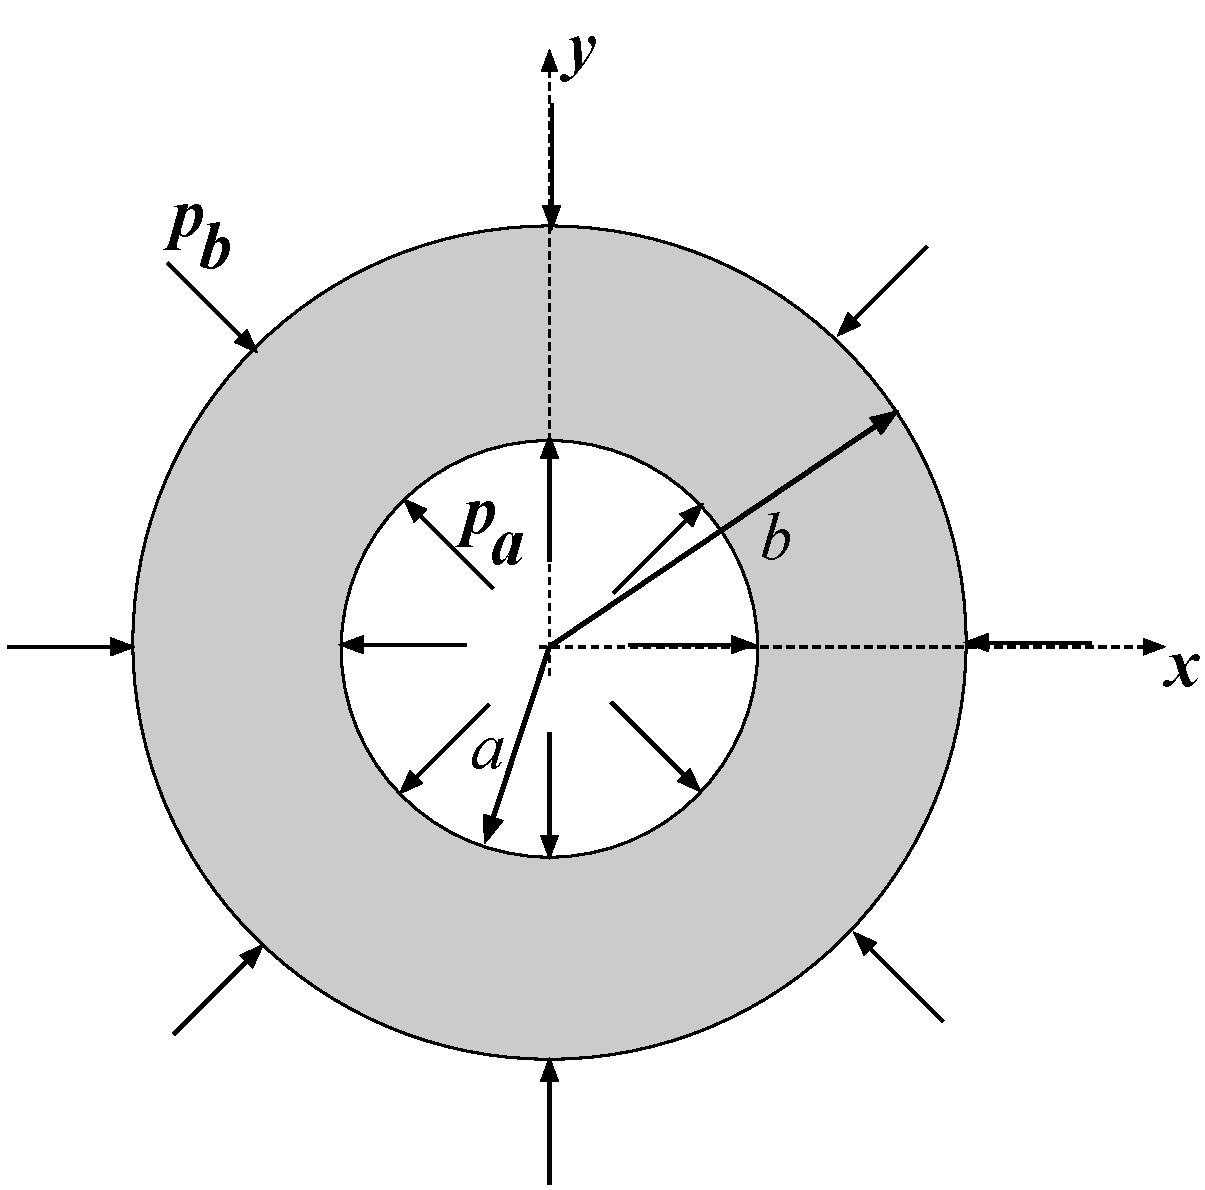
\includegraphics[width=3.0 in]{cilindro.pdf}
	\caption{Cilindro sometido a presión interna $p_a$ y presión externa $p_b$}
	\label{cilindro}
\end{figure}
 	
Usando la solución anterior, y sabiendo que el radio interno es $a$ y radio externo $2a$ determinar el valor máximo que puede tomar la  presión interna $q$ en el cilindro para que el esfuerzo a cortante en los puntos del cilindro que están en contacto con una superficie rígida en su cara externa, tal y como se muestra en la \cref{cilbr}, no superen un valor $\tau=S$. 

\begin{figure}[H]
\centering
	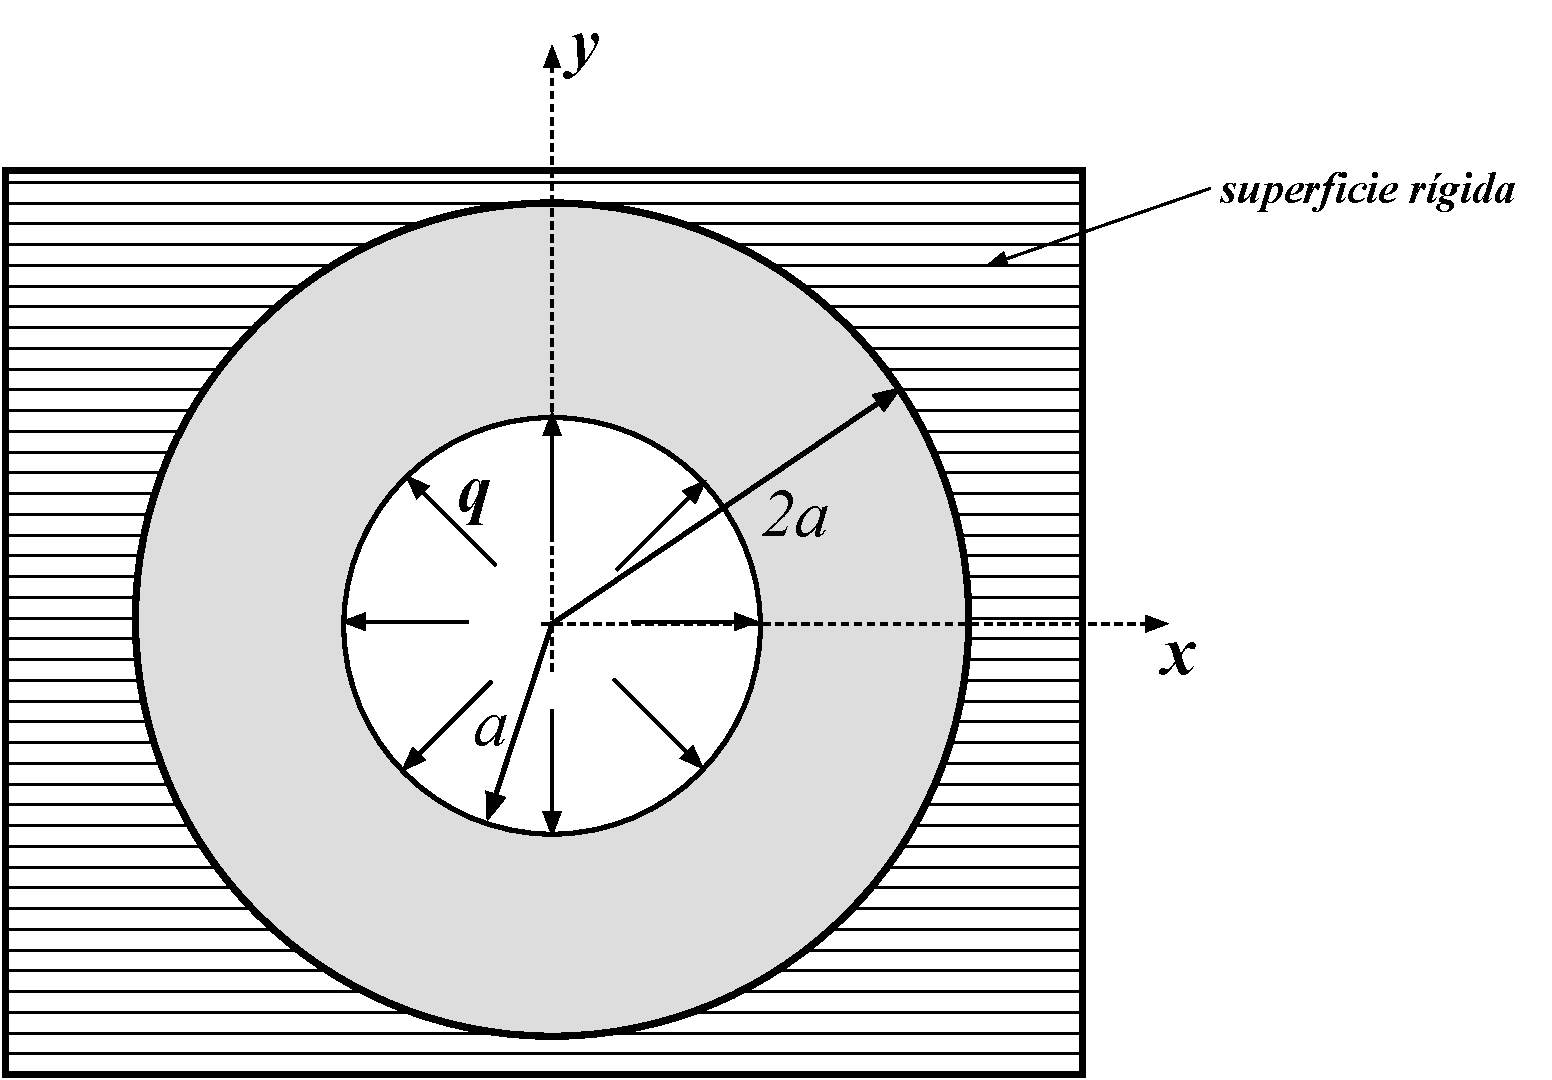
\includegraphics[width=3.5 in]{Cilbase.pdf}
	\caption{Cilindro sometido a presión interna $q$ con superficie rígida en cara externa}
	\label{cilbr}
\end{figure}
%
\textbf{Solución:} \\
sabiendo  que  $b = 2a$ y haciendo el equilibrio de fuerzas que actuarían en las paredes interior y exterior del anillo (pared en contacto con la superficie rígida),  determinemos el valor de $P_b$. 

\begin{equation*}
\begin{split}
{\sum {F}} & = 0 \\
{q  2\pi a} & =  p_b 2\pi 2a \\
{p_b}   & =  \frac{q}{2}
\end{split}
\label{sln1}
\end{equation*}

Haciendo los reemplazos en la solución entregada. Para $\sigma _{rr} $ se tiene: 

\begin{equation*}
\begin{split}
{\sigma _{rr}} &  =  - \frac{{\left( {\frac{{{4a^2}}}{{{r^2}}} - 1} \right)}}{{\left( {\frac{{{4a^2}}}{{{a^2}}} - 1} \right)}}{q} - \frac{{\left( {1 - \frac{{{a^2}}}{{{r^2}}}} \right)}}{{\left( {1 - \frac{{{a^2}}}{{{4a^2}}}} \right)}}\frac{q}{2}\\
{\sigma _{rr}} &  =  - \frac{1}{3}\left( {\frac{{{4a^2}}}{{{r^2}}} - 1} \right) {q} - \frac{4}{3} \left( {1 - \frac{{{a^2}}}{{{r^2}}}} \right)\frac{q}{2}\\
{\sigma _{rr}} &  = \left( - \frac{1}{3} - \frac{{{2a^2}}}{{{3r^2}}} \right) {q} \\\\
\end{split}
\end{equation*}

De forma similar para $\sigma _{\theta\theta} $ se tiene:

\begin{align*}
{\sigma _{\theta\theta}} &  = \left( - \frac{1}{3} + \frac{{{2a^2}}}{{{3r^2}}} \right) {q} \\
\end{align*} 
%
Ahora como nos piden la condición de corte para los puntos sobre la cara externa, es decir cuando $r=2a$, el estado de esfuerzos sería. 

\begin{equation*}
\begin{split}
{\sigma _{rr}} &  = -  \frac{q}{2} \\
{\sigma _{\theta\theta}} &  = \left( - \frac{1}{3} + \frac{{{2a^2}}}{{{12a^2}}} \right) {q} =  -  \frac{q}{6} \\
%{\sigma _{\theta\theta}} &  =  -  \frac{q}{6}\\
{\tau _{r\theta} } &= 0
\end{split}
\end{equation*}

El esfuerzo cortante máximo asociado al plano $r\theta$ está dado por: 

\begin{equation*}
\begin{split}
{\tau } &=  \frac{1}{2}\left( \frac{q}{2} - \frac{q}{6} \right) = \frac{q}{6}   \\
\end{split}
\end{equation*}

Haciendo $\tau = S$, se tiene: 
%
\begin{equation*}
\begin{split}
{q } &=  6S   \\
\end{split}
\end{equation*}

\end{enumerate}

\newpage
\section*{Ejercicios}

%\graphicspath{{imgTen/}} 	% Specifies the directory where pictures are

\begin{enumerate}
  
\item \label{punto01} Si el tensor de esfuerzos en cualquier punto de la cu\~na
presentada en la \cref{figure4} es:\\
	\\
	%
	$[\sigma] = \left[ \begin{array}{ccc}
	-S cot \phi & 0 \\ 
	0 & S tan \phi
	\end{array}  \right] $\\
	%
	\begin{figure}[H]
		\centering
		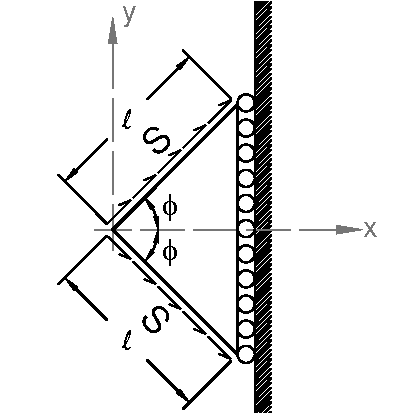
\includegraphics[height=6.25cm]{Ejer4_1.pdf}
		\caption{Cuña de espesor $e$ sometida a tensiones tangenciales constantes $(S)$ en dos caras.}
		\label{figure4}
	\end{figure}
	%
	\begin{enumerate}
		\item Verificar el equilibrio global $\left( \sum F = 0.0 \right)$.
		\item Verificar el equilibrio a nivel diferencial.
		\item  \textquestiondown Es posible encontrar esfuerzos cortantes $\tau_{xy}$ al interior de la cu\~na mayores a $S$?. Responder s\'i o no y justificar su respuesta.
		\item Calcule el vector de tensiones en cada cara de la cu\~na. 
	\end{enumerate}



\item \label{punto03}  En la \cref{barra:colga1} se muestra un elemento
con densidad $\rho$, de secci\'on circular, soportado de su extremo superior y est\'a sometido solamente a la acci\'on de su peso propio. Se indica el tensor de esfuerzos en el sistema coordenado $x-y$ para los puntos a y b mostrados en la figura.\\
	%
	\\
	Punto a: $[\sigma] = \left[ \begin{array}{ccc}
	0 & 0\\ 
	0 & 2 \gamma L/3\\
	\end{array}  \right] $
	\hspace{30mm}
	Punto b: $[\sigma] = \left[ \begin{array}{ccc}
	0 & 0\\ 
	0 & \gamma L/3\\
	\end{array}  \right] $ \\\\
	%
	\begin{figure}[H]
		\centering
		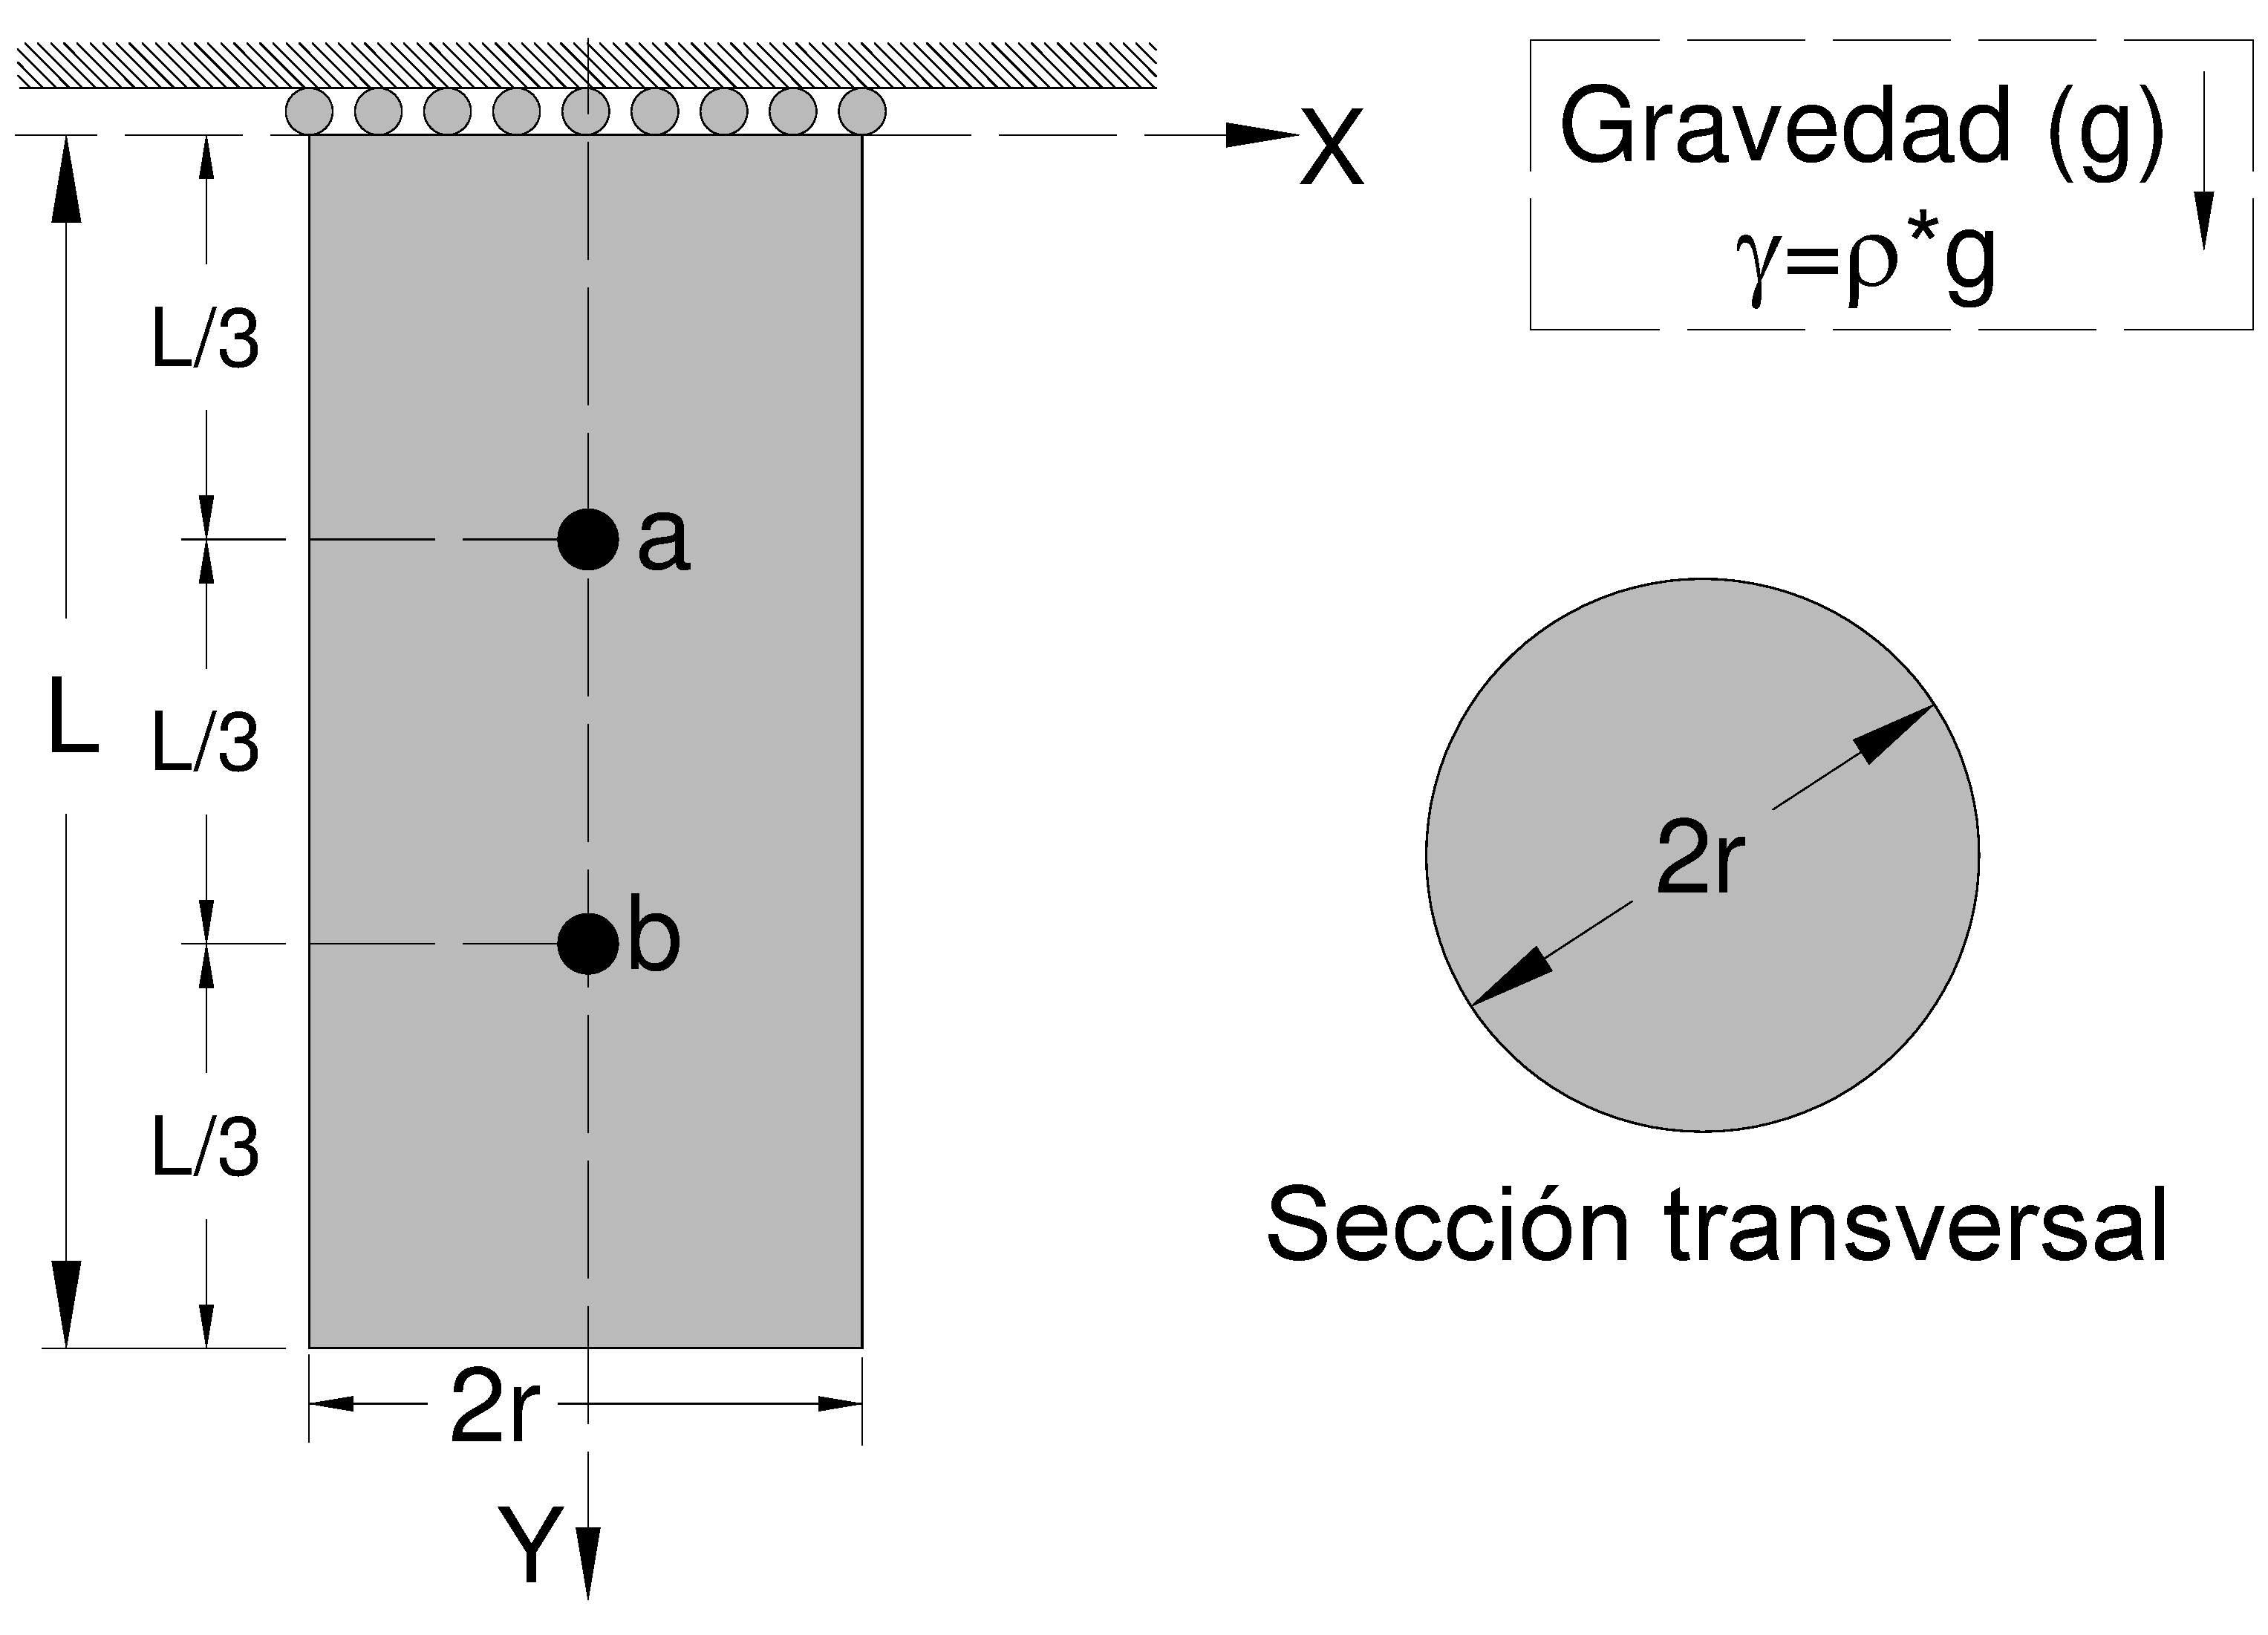
\includegraphics[height=5.75cm]{Ejer4_3.pdf}
		\caption{Barra colgada}
		 \label{barra:colga1}
	\end{figure}
	%
	Si el tensor de esfuerzos var\'ia de forma lineal a lo largo del eje $y$, se pide:
	%
	\begin{enumerate}
	% 
		\item El  tensor de esfuerzos para cualquier punto al interior del elemento. 
		\item \textquestiondown El elemento se encuentra en equilibrio a nivel diferencial?. Justifique su respuesta matem\'aticamente.
		\item Si el elemento es infinitamente resistente ante esfuerzos de tracci\'on y de compresi\'on, pero su capacidad m\'axima ante esfuerzos cortantes est\'a dada por \begin{large} $\tau_{max}$ \end{large}. Determine:
	%
		\begin{enumerate} 
			\item \textquestiondown Cu\'al es la longitud m\'axima posible del elemento?. 
			\item  \textquestiondown Cu\'al es la fuerza en el soporte superior cuando se produce la falla por corte?.
			\item \textquestiondown Cu\'al es la tensi\'on en la secci\'on transversal inferior del elemento  $\left( y=L \right)$  cuando se produce la falla por corte?.
		\end{enumerate}
%
		\item 	Si el elemento es infinitamente resistente ante esfuerzos cortantes y de compresi\'on, pero su capacidad m\'axima ante esfuerzos de tracci\'on est\'a dada por \begin{large} $\sigma_{trac}$ \end{large}. Determine:
		\begin{enumerate} 
			\item \textquestiondown Cu\'al es la longitud m\'axima posible del elemento?. 
			\item \textquestiondown Cu\'al es la tensi\'on en la secci\'on transversal inferior del elemento  $\left( y=L \right)$  cuando se produce la falla por tracci\'on?. 
			\item \textquestiondown Cu\'al es la fuerza en el soporte superior cuando se produce la falla por tracci\'on?.
		\end{enumerate}	
	
		\item	Si el elemento es infinitamente resistente ante esfuerzos cortantes y de tracci\'on, pero su capacidad m\'axima ante esfuerzos de compresi\'on est\'a dada por \begin{large} $\sigma_{comp}$ \end{large}. Determine: 
		\begin{enumerate}		
			\item \textquestiondown Cu\'al es la longitud m\'axima posible del elemento?. 
			\item \textquestiondown Cu\'al es la tensi\'on en la secci\'on transversal inferior del elemento  $\left( y=L \right)$  cuando se produce la falla por compresi\'on?. 
			\item \textquestiondown Cu\'al es la fuerza en el soporte superior cuando se produce la falla por compresi\'on?.
		\end{enumerate}
	\end{enumerate}


\item \label{punto04} El tensor de tensiones de un medio continuo se describe
con la siguiente di\'adica:
		\[ [\sigma] = \left[ \begin{array}{ccc}
		-2x^2yx & 4z^2+yx & 2z^2yx-xz \\ 
		4z^2+yx & yz+4y^2 & -yz-xyz \\ 
		2z^2yx-xz & -yz-xyz & 4z^3
		\end{array}  \right] \enspace\]
		%
	\begin{enumerate}
		\item Calcular la fuerza de cuerpo necesaria para mantener el medio continuo en equilibrio est\'atico.
%		\item Calcular la fuerza de cuerpo necesaria para mantener el medio continuo en equilibrio din\'amico si se tiene el campo de velocidades $v_x=xt$, $v_y=xy$ y $v_z=zt$.
	\end{enumerate}
% *************************** %
\item \label{punto05} Si en un medio continuo, el campo de tensiones est\'a dado
por el tensor:
		\[ [\sigma] = \left[ \begin{array}{ccc}
		x^2y & (1-y^2)x & 0 \\ 
		(1-y^2)x & (y^3-3y)/3 & 0 \\ 
		0 & 0 & 2z^2
		\end{array}  \right]\enspace \]
		%
	Determinar:
	%
	\begin{enumerate}
		\item La fuerza de cuerpo necesaria para mantener el medio continuo en equilibrio est\'atico.
		\item Las tensiones principales en el punto $P(a,0,0)$.
		\item La tensi\'on tangencial (corte) m\'axima en el punto $P$.
%		\item Las fuerzas de cuerpo necesarias para que se cumpla el equilibrio din\'amico si se tiene el campo de velocidades $v_x=xy$, $v_y=x^2t$ y $v_z=xyzt$.
	\end{enumerate}
% *************************** %

% *************************** %


\item \label{punto07} El campo del tensor de tensiones de Cauchy viene
representado por sus componentes como:
		\[[\sigma] = k\left[ \begin{array}{ccc}
		x_1^2 x_2 & (a^2-x_2^2)x_1 & 0 \\ 
		(a^2-x_2^2)x_1 & \frac{1}{3}(x_2^3 - 3a^2 x_2) & 0 \\ 
		0 & 0 & 2ax_3^2
		\end{array}  \right] \enspace,\]
%	
	donde $k$ y $a$ son constantes.
%
	Encontrar el campo de fuerzas de cuerpo $\mathbf{b}$ (por unidad de volumen) necesario para que el sistema est\'e en equilibrio.
%


\item  \label{punto16}   En las \cref{SolucionP} y \cref{Solucionw} se muestra las soluciones para una masa de suelo sometido a una carga superficial $P$ y una carga distribuida uniforme superficial $w$ .  Los esfuerzos al interior del suelo debidos a la carga $P$ y $w$, en un sistema  coordenado cilíndrico $\left(r,{\theta},z \right)$, est\'an dados: \\\\
%
%\begin{large}
%\centering
$[\sigma]_P = -\dfrac{2P}{\pi r} \left[ \begin{array}{ccc}
\cos\theta & 0 & 0\\ 
0 & 0 & 0\\
0 & 0 & 0\\
\end{array}  \right] $
\hspace*{5mm}
$[\sigma]_w = -\dfrac{w}{\pi} \left[ \begin{array}{ccc}
\pi + 2\theta - \sin \left(2\theta \right)  & 1 -\cos \left(2\theta\right) & 0\\ 
1 - \cos \left(2\theta \right)  & \pi + 2\theta + \sin \left(2\theta \right) & 0\\
0 & 0 & 0\\
\end{array}  \right] $
%\end{large}

Donde $P$ y $w$ son las cargas, $\theta$ es el ángulo medido desde la vertical y positivo en sentido antihorario. 
%
\begin{figure}[H]
	\centering
		\subfloat [Soluci\'on carga vertical $P$]{ 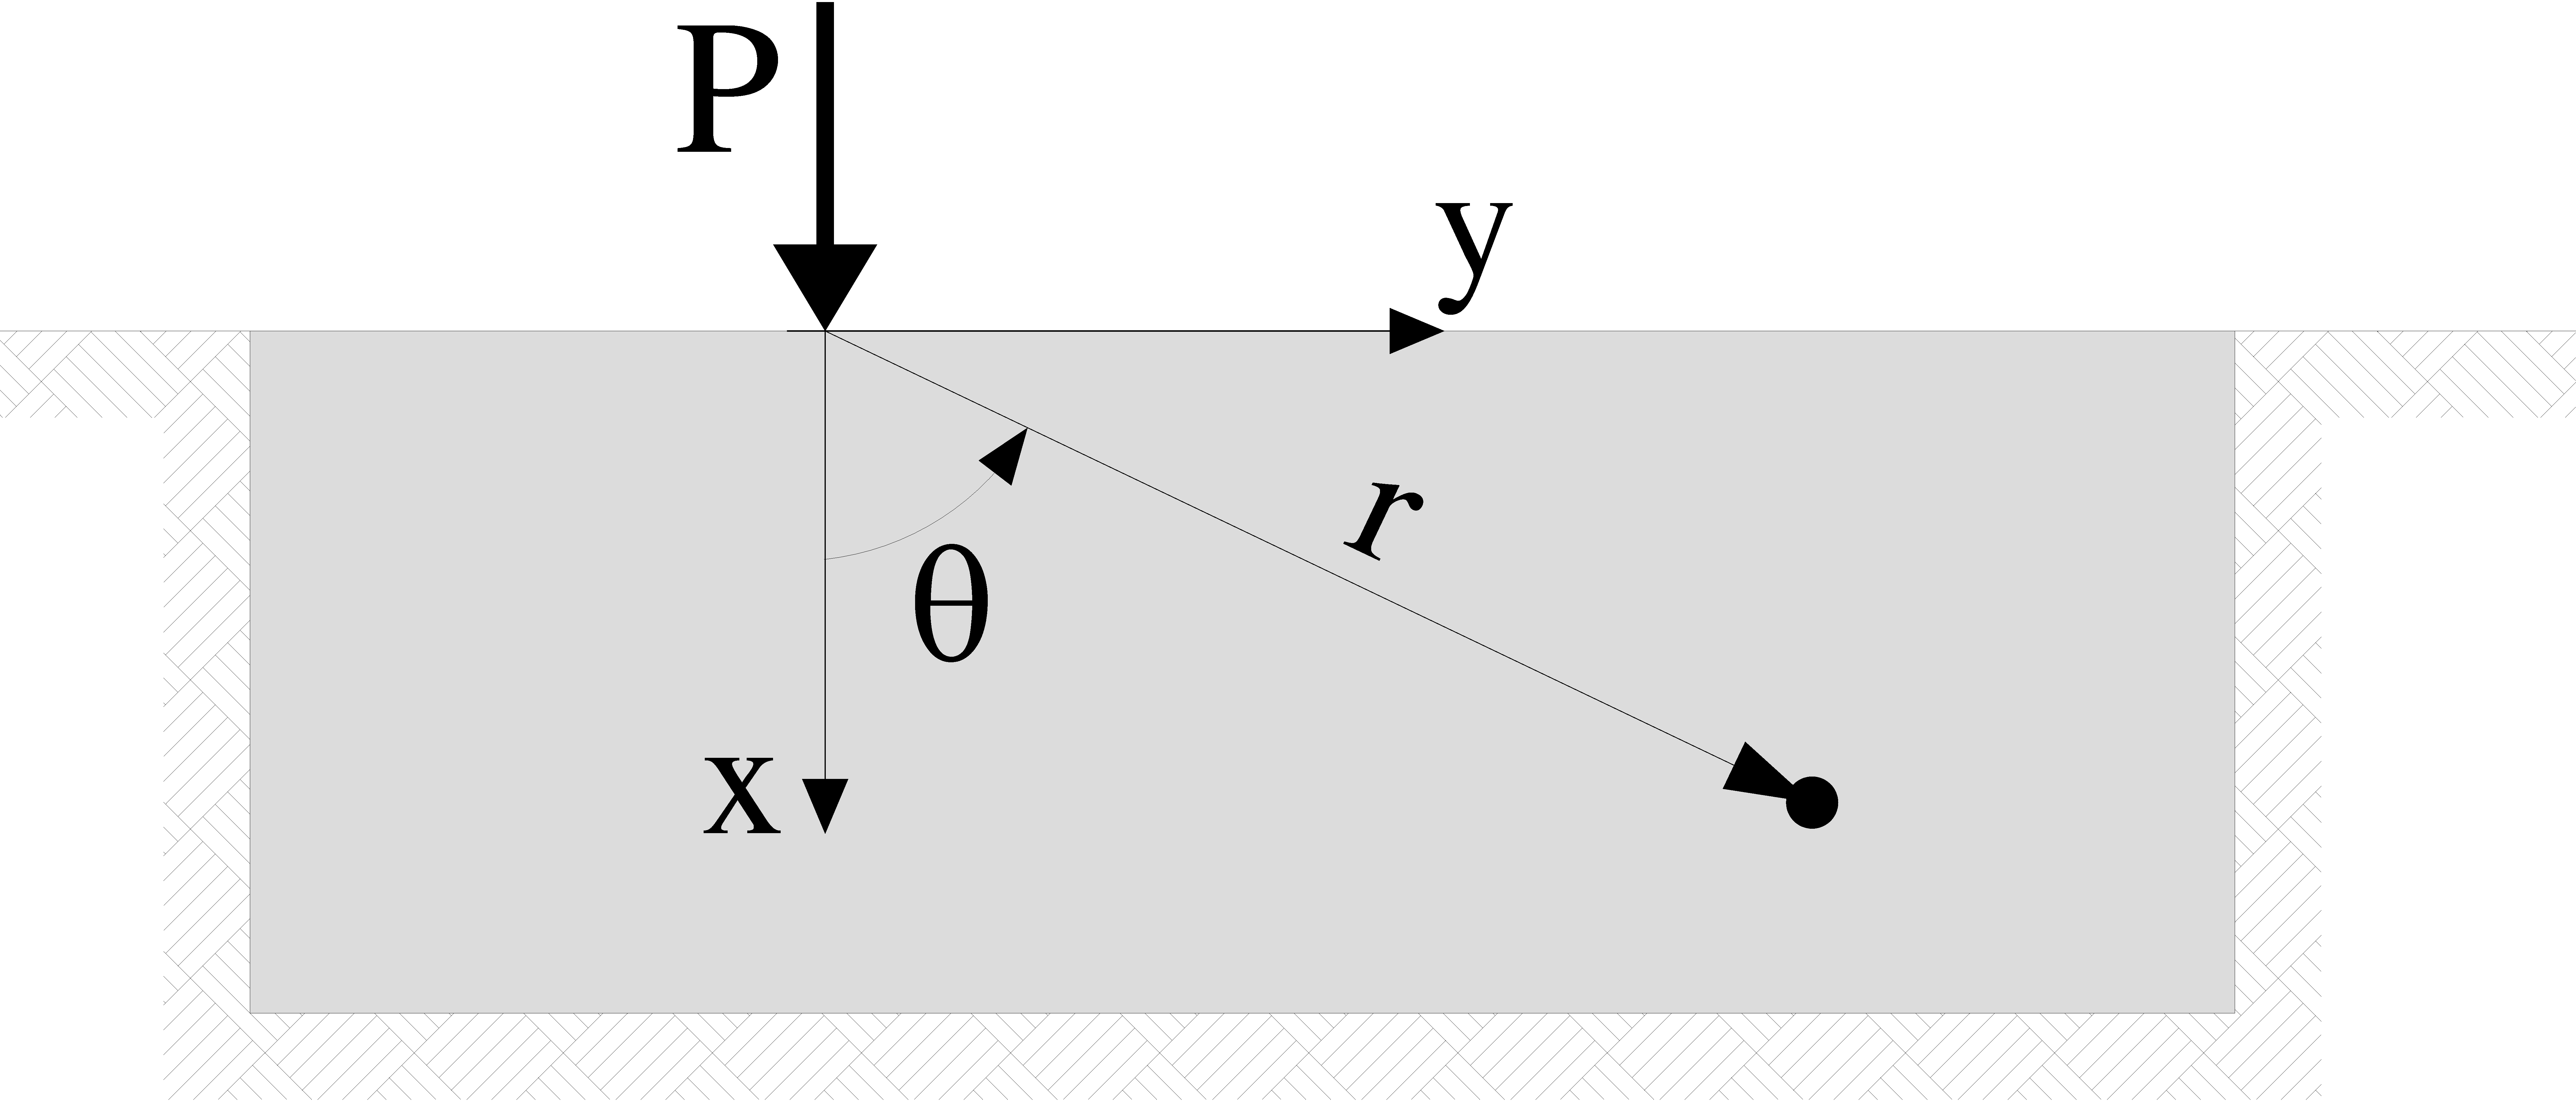
\includegraphics[width=3.0in]{Ejer4_16_1.pdf}\label{SolucionP}}
		\hspace{1.0cm}
		\subfloat [carga uniforme superficial $w$]{ 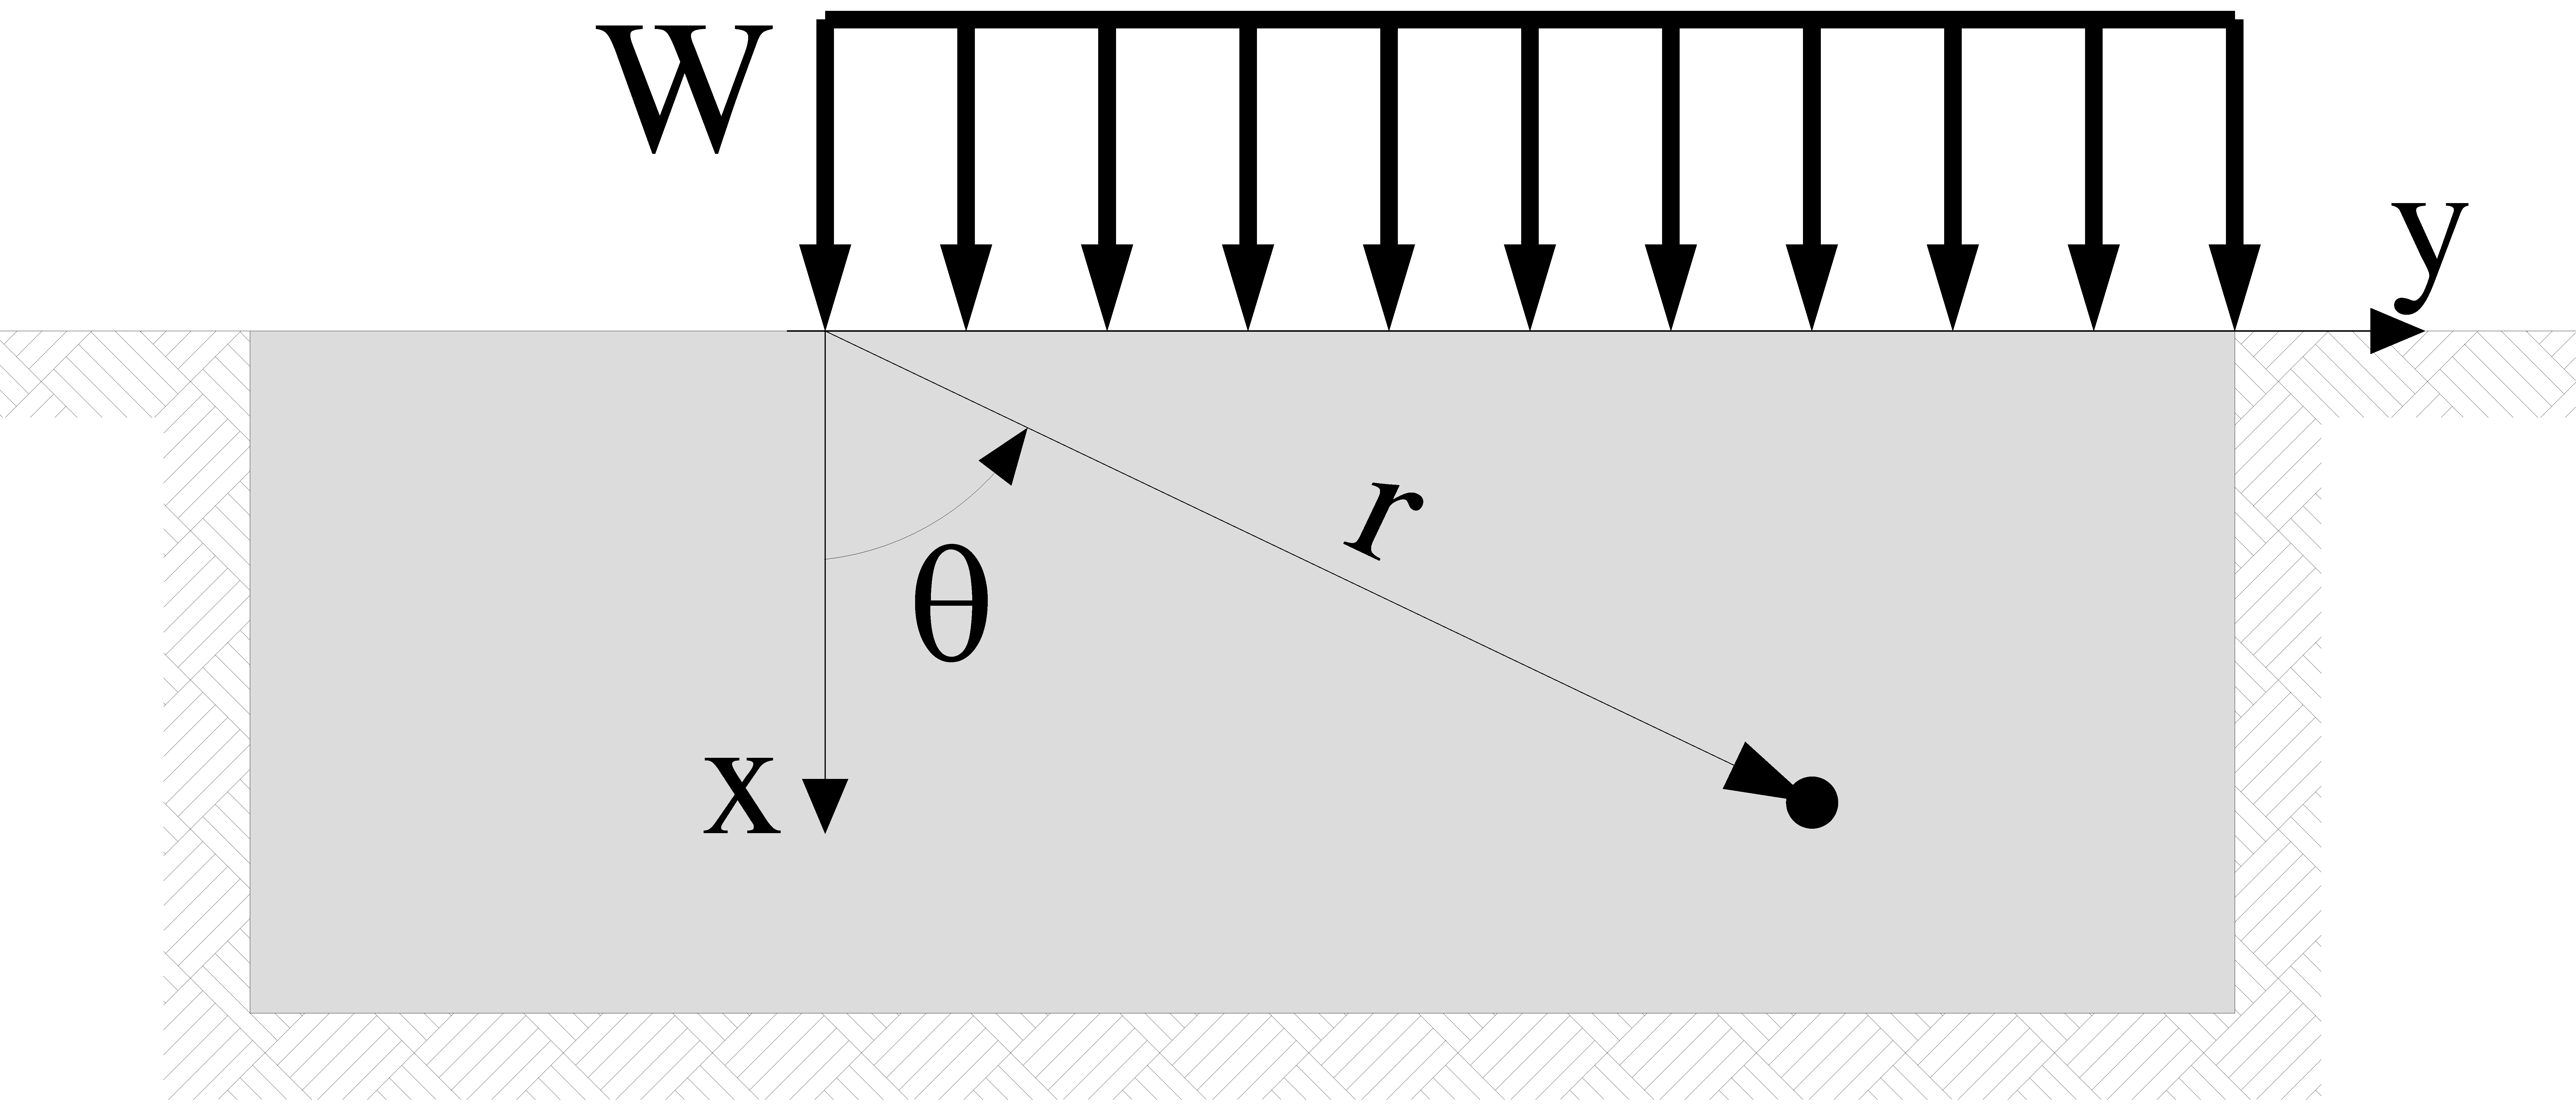
\includegraphics[width=3.0in]{Ejer4_16_2.pdf}\label{Solucionw}}		
	\caption{Soluciones fundamentales}
	\label{solucionpw} 
\end{figure}
%
Si a la masa de suelo se transmiten de manera simúltanea las cargas $P=100$ $Ton/m $ y $w= (100 + tiempo)$ $Ton/m^2$, y se quiere instalar un sistema de acueducto conformado por dos tuberías A y B (de díametro despreciable) perpendicular al plano mostrado ($XY$), en donde la profundad para la tubería A es $H_{A} = 1.0 / \pi$ $m$ y para la tubería B  es $H_{B} = 0.75 H_{A}$ tal y como se muestra en la \cref{cargasPw}. Determine:
%		
\begin{figure}[H]
	\centering
	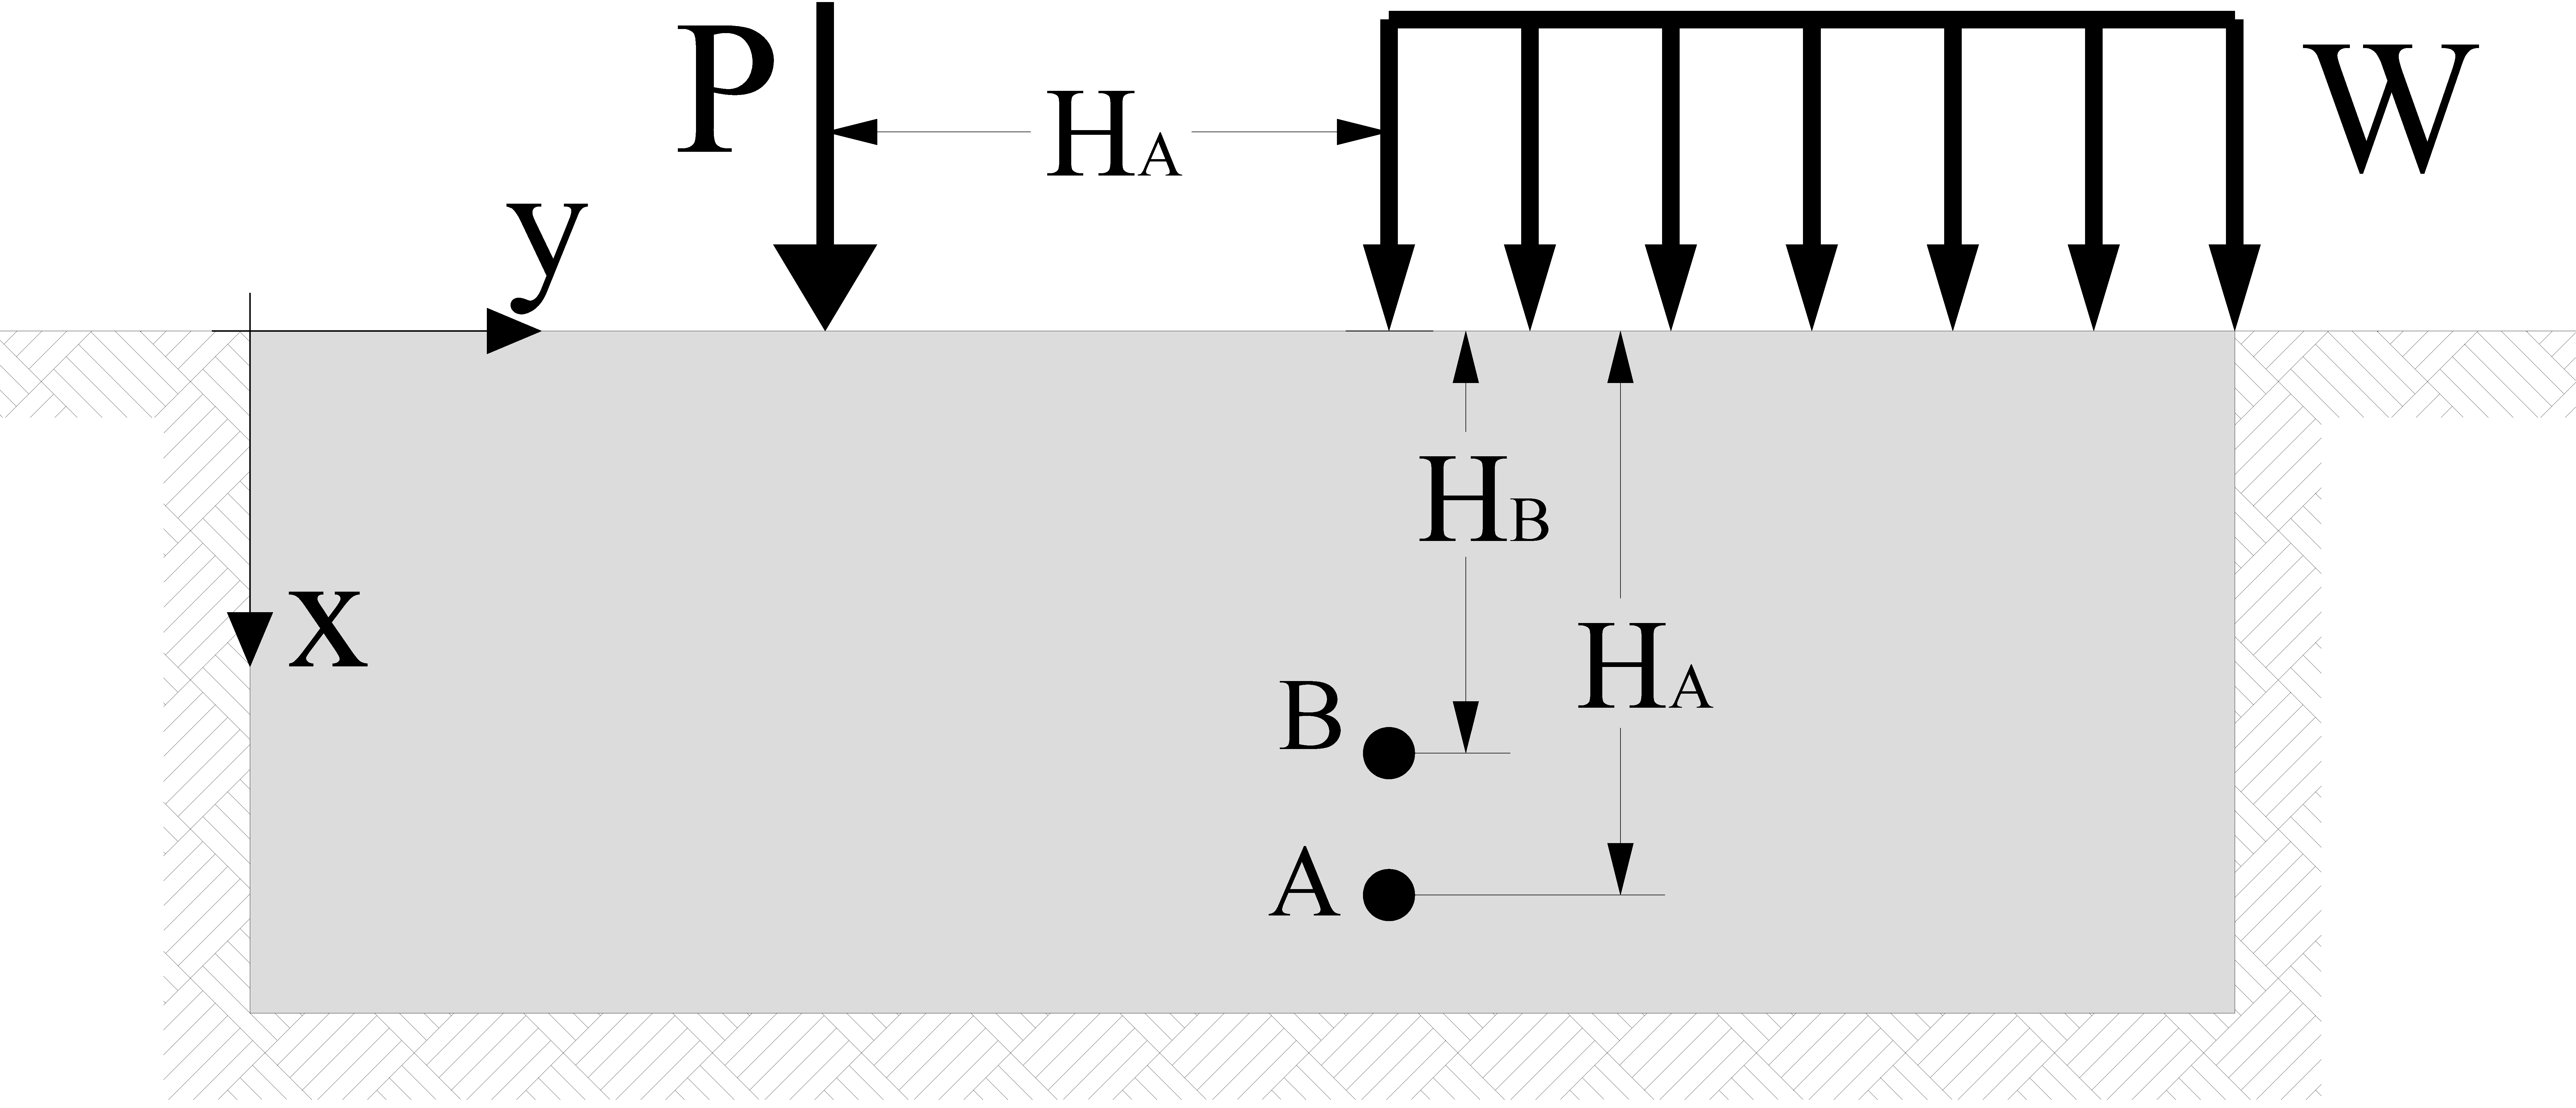
\includegraphics[width=3.5in]{Ejer4_16_3.pdf} 
	\caption{Cargas y tuber\'ias}
	\label{cargasPw}
\end{figure}
%
\begin{enumerate}
	\item  Determine cuál tubería falla primero y en que tiempo se produce la falla, si se sabe que el material de la tubería A es infinitamente resistente a esfuerzos cortantes pero no soporta esfuerzos axiales mayores o iguales a $210,5\dfrac{Ton}{m^2}$  y el material de la tubería B es infinitamente resistente a esfuerzos axiales pero no sorporta esfuerzos cortantes mayores o iguales a $100,25\dfrac{Ton}{m^2}$. 
\end{enumerate}
\newpage
\item \label{punto17}  En la \cref{barra} se presenta una barra de radio $C$ y longitud $L$. El estado de esfuerzos del  medio continuo en el sistema cartesiano $x,y,z$ est\'a dado por el tensor: \\\\
%
\begin{equation}
\begin{aligned}
& \sigma_{xx} = 0; \hspace*{5mm}  \sigma_{yy} = 0; \hspace*{5mm}  \sigma_{zz} = 0; \\
&\tau_{xy} = 0; \hspace*{5mm}  \tau_{xz} = {\omega}y;	\hspace*{5mm} \tau_{zy} = - {\omega}x \\
\end{aligned}
\label{trans}
\end{equation}
%
\begin{figure}[H]
	\centering
	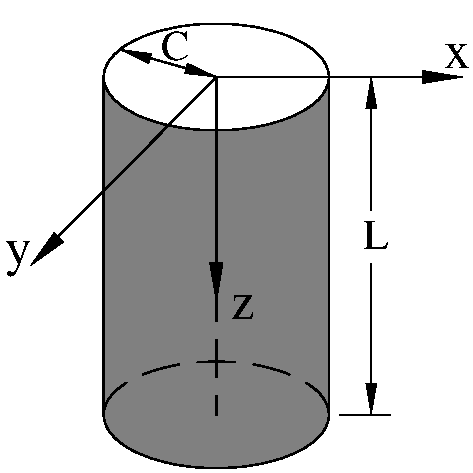
\includegraphics[height=5cm]{Ejer4_17.pdf} 
	\caption{Medio Continuo}
	\label{barra}
\end{figure}
%
Donde $\omega$ es una constante.\\
\begin{enumerate}
	\item  Determine el valor del m\'aximo esfuerzo de compresi\'on al que está sometido la barra y la ubicaci\'on (coodenadas de los puntos) donde se presentan esos valores máximos. 
    \item ¿Describa que problema resuelve el estado de esfuerzos en a barra?  \textsl{Sugerencia: para facilitar el an\'alisis estudie las caras con vector normal en direcci\'on z.} 
	\item Si el cuerpo tiene longitud $L = 50 cm$, $\omega = 5000 \; Tonf / m^3$, adem\'as es infinitamente resistente ante esfuerzos de tracci\'on y de compresi\'on, pero su capacidad m\'axima ante esfuerzos tangenciales es  $ \tau_{max} = 88 \; kgf/cm^2$.  Determine el valor m\'aximo del radio $C$ que podr\'ia tener el cuerpo. 
\end{enumerate}


\end{enumerate}
\end{document}


